% ****** Start of file aipsamp.tex ******
%
%   This file is part of the AIP files in the AIP distribution for REVTeX 4.
%   Version 4.1 of REVTeX, October 2009
%
%   Copyright (c) 2009 American Institute of Physics.
%
%   See the AIP README file for restrictions and more information.
%
% TeX'ing this file requires that you have AMS-LaTeX 2.0 installed
% as well as the rest of the prerequisites for REVTeX 4.1
%
% It also requires running BibTeX. The commands are as follows:
%
%  1)  latex  aipsamp
%  2)  bibtex aipsamp
%  3)  latex  aipsamp
%  4)  latex  aipsamp
%
% Use this file as a source of example code for your aip document.
% Use the file aiptemplate.tex as a template for your document.
\documentclass[
aip,
%jmp,%
%bmf,%
%sd,%
rsi,%
%jcp,
amsmath,amssymb,
%preprint,%
reprint,%
%author-year,%
%author-numerical,%
]{revtex4-1}

\usepackage{graphicx}% Include figure files
\usepackage{dcolumn}% Align table columns on decimal point
\usepackage{bm}% bold math
%\usepackage[mathlines]{lineno}% Enable numbering of text and display math
%\linenumbers\relax % Commence numbering lines

\usepackage[T1]{fontenc}
\usepackage[utf8]{inputenc}
\usepackage[polutonikogreek,english]{babel}
\usepackage{hyperref}
\hypersetup{colorlinks=true,allcolors=blue}
\usepackage[all]{hypcap}

\newcommand{\micron}{\textgreek{μ}m}
\newcommand{\microsec}{\textgreek{μ}s}
\newcommand{{\usalex}}{\textgreek{μ}sALEX}

\begin{document}

\preprint{}

\title[48-spot smFRET-PAX setup]{48-spot single-molecule FRET setup with periodic acceptor excitation}

\author{Antonino Ingargiola}
\email{ingargiola.antonino@gmail.com}
\author{Maya Segal}
\affiliation{
Department of Chemistry and Biochemistry, University of California Los Angeles, USA}
\author{Angelo Gulinatti}
\author{Ivan Rech}
\author{Ivan Labanca}
\affiliation{
Dipartimento di Elettronica, Informazione e Bioingegneria , Politecnico di Milano, Milan, Italy
}
\author{Piera Maccagnani}
\affiliation{Istituto per la Microelettronica e Microsistemi, IMM-CNR, Bologna, Italy.}
\author{Massimo Ghioni}
\affiliation{
Dipartimento di Elettronica, Informazione e Bioingegneria , Politecnico di Milano, Milan, Italy
}
\author{Shimon Weiss}
\author{Xavier Michalet}
 \email{michalet@chem.ucla.edu}
\affiliation{
Department of Chemistry and Biochemistry, University of California Los Angeles, USA}


\date{\today}% It is always \today, today,

\begin{abstract}
Single-molecule FRET (smFRET) allows measuring distances between donor and
acceptor fluorophores on the 3-10~nm range.
Solution-based smFRET allows measurement of binding-unbinding events
or conformational changes of dye-labeled biomolecules without ensemble averaging
and free from surface perturbations. When employing dual (or multi)
laser excitation,
smFRET allows resolving the number of fluorescent
labels on each molecule, greatly enhancing the ability to study
heterogeneous samples.
A major drawback to solution-based smFRET is the low throughput,
which renders repetitive measurements expensive and hinders the ability
to study kinetic phenomena in real-time.

Here we demonstrate a high-throughput smFRET system which
multiplexes acquisition by using 48 excitation spots and two
48-pixel SPAD array detectors. The system employs two excitation lasers
allowing separation of species with one or two active fluorophores.
The performance of the system is demonstrated on a set of doubly-labeled
double-stranded DNA oligonucleotides
with different distances between donor and acceptor dyes along the DNA duplex.
We show that the acquisition time for accurate subpopulation identification
is reduced from several minutes to seconds, opening the way
to high-throughput screening applications and
real-time kinetics studies of enzymatic reactions such as DNA transcription
by bacterial RNA polymerase.
\end{abstract}

\keywords{Single-molecule FRET, high-throughput, SPAD array}
%Use showkeys class option if keyword display desired
\maketitle

\section{Introduction} \label{sec:intro}

Detailed knowledge of the three-dimensional (3D) atomistic structure of
macromolecular complexes is essential to understand their
biological function. For decades, X-ray crystallography and nuclear
magnetic resonance (NMR) spectroscopy have been the techniques of choice
for obtaining atomically resolved macromolecular structures. More recently,
single-particle cryo-electron microscopy (cryo-EM) has complemented these
methods for determination of large macromolecular structures with the
added ability to classify different conformations. However, macromolecules
spontaneously and dynamically explore various conformations in equilibrium
that are hard to capture by the above-mentioned methods. Understanding the
functional roles of these structures requires a full dynamic picture.
Single-molecule Förster resonance energy transfer
(smFRET)~\cite{dahan_ratiometric_1999}
has paved the way
for studying such structural dynamics in biologically-relevant conditions.
smFRET allows determination of each conformational state that may exist in
an ensemble of macromolecular complexes as well as the distance between
specific residues for each
state~\cite{chakraborty_opening_2012,kapanidis_initial_2006,kapanidis_retention_2005,ha_single-molecule_1999,deniz_single-pair_1999}.
Recently, several groups have implemented smFRET to
measure distances between multiple different pairs of residues to
construct 3D macromolecular structures of distinct conformations by
triangulation and comparison with existing X-ray crystal
structures~\cite{dimura_quantitative_2016,hellenkamp_multidomain_2017,hoefling_structural_2011,kalinin_toolkit_2012,muschielok_nano-positioning_2008,muschielok_application_2011}.
Moreover, smFRET can measure the time-evolution of various
distances between multiple FRET pairs, and hence report upon the dynamic
3D structure of a macromolecule undergoing conformational changes.
Thus far, due to the requirement of low sample concentration imposed
by the necessity to have no more than one molecule within the
diffraction-limited confocal volume at a given
time~\cite{dahan_ratiometric_1999,fries_quantitative_1998},
only very slow kinetics can be measured. Therefore, increased throughput
is essential for both static and dynamic measurements of multiple distances.

To overcome
this limitation, we recently introduced a multispot excitation scheme taking
advantage of novel single-photon avalanche diode (SPAD)
arrays~\cite{ingargiola_parallel_2012,ingargiola_8-spot_2013,ingargiola_multispot_2017}.
We demonstrated that the resulting setup indeed allowed acquisition of
single-molecule data comparable to that of standard single-spot
setups, but with a throughput that scaled linearly with the number
of excitation spots.
We illustrated an application of this enhanced throughput
by measuring the bubble closing kinetics during promoter escape in bacterial
transcription~\cite{ingargiola_multispot_2017}.
While encouraging, these results were partially unsatisfactory because they
were obtained with only 8 spots and also because
the setup only incorporated a single laser, used for continuous excitation of the
donor dye of the FRET pair~\cite{ingargiola_multispot_2017}.
Single-laser smFRET is unable to distinguish low FRET molecules
(molecules with active donor (D) and acceptor (A) dyes in which the D-A distance is
large compared to the Förster radius) from D-only molecules
(i.e. molecules with a single donor, or dually-labeled molecules
with an inactive or bleached acceptor).
As the latter categories are present in most samples,
it is important to identify and separate them from low FRET molecules
of interest.

To address this problem, \emph{Microsecond Alternated Laser EXcitation}
smFRET (referred throughout as {\usalex} for brevity), was
introduced several years ago~\cite{kapanidis_fluorescence-aided_2004,kapanidis_alternating-laser_2005},
and later extended to pulsed laser excitation schemes
(nsALEX~\cite{laurence_probing_2005} or PIE~\cite{muller_pulsed_2005}).
Briefly, in {\usalex},
two excitation lasers are alternated on and off every few tens of
{\microsec} allowing separation of species with only a single active
dye, i.e. D-only and A-only populations, from doubly-labeled species with both dyes
active, the FRET populations. Indeed, only FRET populations
emit a fluorescence signal during both D-excitation laser  (due to
excitation of the donor) and  A-excitation laser  (due to excitation
of the acceptor).
This, in turn, extends the number of FRET sub-populations that can be reliably
identified within a sample in the regime of low mean FRET efficiencies, 
referred to throughout as ``low FRET''.
This scheme has since been extended to up to 4 laser excitations, allowing
powerful molecular sorting applications~\cite{lee_three-color_2007,yim_four-color_2012}.
A simplified version of this laser alternation principle was presented in
ref.~\onlinecite{doose_periodic_2007}, where the D-excitation laser
is left on at all times while the A-excitation laser is alternated.
This Periodic Acceptor eXcitation single-molecule FRET
technique~\cite{doose_periodic_2007}, referred to as PAX for brevity, simplifies
the optical setup while maintaining the advantages of {\usalex}, namely
the ability to determine the number of D and A dyes in each detected molecule
or to simplify the extraction of accurate FRET efficiency values~\cite{lee_accurate_2005}.
Here we present a significant improvement to our original multispot
setup by (i) introducing a 48-spot illumination and detection scheme,
and (ii) implementing a 2-lasers, PAX illumination approach.

This paper is organized as follows.
In Section~\ref{sec:setup_brief} we briefly introduce the optical setup,
the detectors (Section~\ref{sec:detectors}) and the modulation scheme
(Section~\ref{sec:48spot-pattern}). In Section~\ref{sec:smfret-meas} we
report single-molecule measurements, starting with a brief
description of the data analysis (Section~\ref{sec:analysis}).
To demonstrate the uniformity across spots, we study
the burst peak photon rate (Section~\ref{sec:peak-phrate})
and E-S histograms (Section~\ref{sec:EShist}).
Finally, we compare single-spot {\usalex} and 48-spot PAX measurements
(Section~\ref{sec:alexpax-comp} ). We conclude with a brief summary and perspective in Section
~\ref{sec:conclusion}.

\subsection{Software and data availability}
Software used to operate the multispot setup (including
LCOS-SLM pattern generation, LabVIEW-FPGA time-stamping code,
piezo-motor control, etc.) is provided in different repositories
 available on GitHub at
\href{https://github.com/multispot-software}{https://github.com/multispot-software}.
Software used for data analysis can be found in the
\href{https://github.com/tritemio/48-spot-smFRET-PAX-analysis}{48-spot-smFRET-PAX-analysis}
repository. Links to specific analysis notebooks are added in the caption of each
figure. Data files are publicly available on
Figshare~\cite{ingargiola_datasets_2017}.


\begin{figure*}
    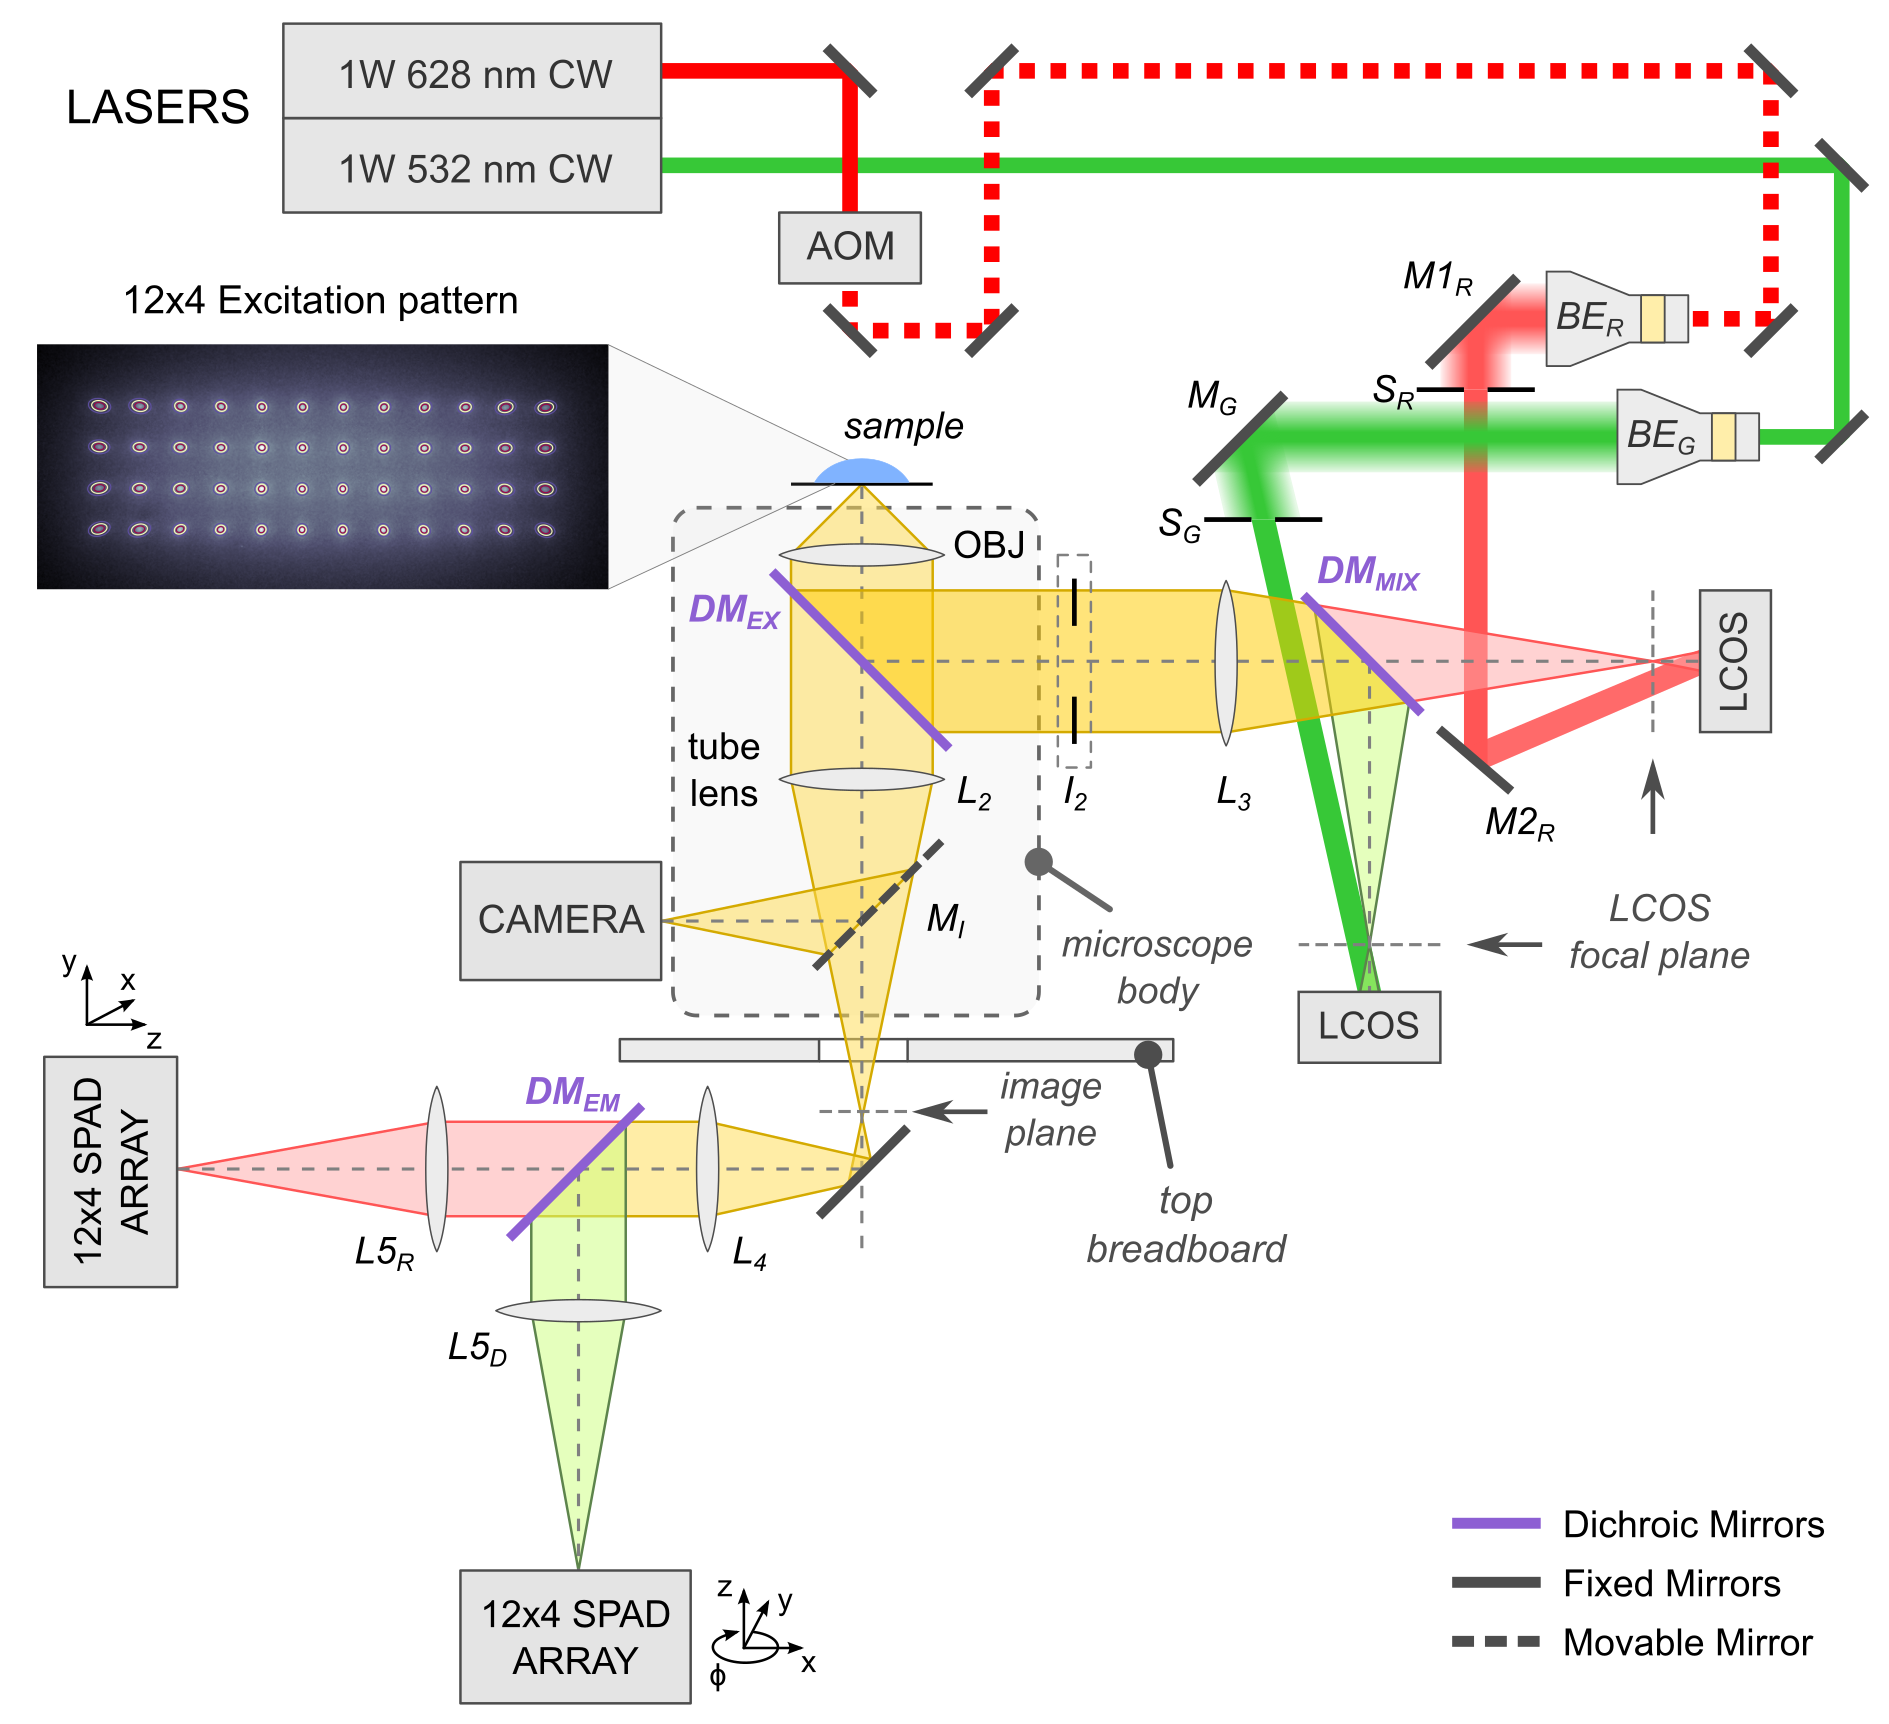
\includegraphics[width=0.7\textwidth]{figures/design_multispot_LCOS_camera_SPAD}
    \caption{{\label{fig:setup} Schematic of the 48-spot PAX setup. The lasers and detectors are on the main optical table, while the microscope (enclosed in the dashed box), beam expanders, and LCOS-SLMs are located on a raised breadboard. See
    main text and Appendix~\ref{sec:setup} for a detailed description.}}
\end{figure*}

\section{Setup description}
\label{sec:setup_brief}

In this Section, we provide a brief description of the setup.
A more detailed description can be found in
Appendix~\ref{sec:setup}, while details of laser and SPAD array
alignment can be found in Appendix~\ref{sec:laseralign}
and~\ref{sec:spadalign}.

A schematic of the setup is shown in Fig.~\ref{fig:setup}.
The setup includes two 1 W CW excitation lasers (green: 532~nm, red: 628~nm)
where only the red laser is modulated via an acoustic-optic modulator (AOM).
After polarization adjustment and beam expansion, the two lasers
are phase modulated by their respective LCOS-SLM, generating two
48-spot patterns on an image plane in front of each LCOS-SLM (\emph{LCOS image plane}).
The two modulated laser beams are then combined by a dichroic mirror ($DM_{MIX}$) and
recollimated ($L_3$) before being focused into the sample by a
high numerical aperture (NA) water immersion objective lens (60X, NA = 1.2, Olympus, Waltham, MA).
Emitted fluorescence is collected by the  objective lens,
separated from the excitation wavelengths by a dual-band polychroic mirror ($DM_{EX}$),
and focused by a tube lens ($L_2$) into the microscope's bottom image plane.
Next, emitted fluorescence light is recollimated ($L_4$), separated into donor
and acceptor spectral bands by a dichroic mirror ($DM_{EM}$), and focused into two different
48-pixel SPAD arrays mounted on motorized micro-positioning stages (xyz vectors).
The system is aligned such that each SPAD is optically
conjugated to one excitation spot in the sample.

Output from the detectors (one TTL pulse train per SPAD) is processed by a
field-programmable gate array (FPGA) equipped board (PXI-7813R, National Instruments, Austin, TX) 
that performs photon time-stamping with 12.5~ns resolution and transfers data 
asynchronously to the host PC.
The host PC runs a LabVIEW acquisition software, which displays the binned signal recorded from all 96-channels in real-time as 96 color-coded time traces, implements alignment routines, and saves the data to
disk. After data acquisition, file conversion to the photon-HDF5 format~\cite{ingargiola_photon-hdf5:_2016-1} and analysis is performed on a second PC, therefore allowing non-stop acquisition of sequential files.

\subsection{Detectors}
\label{sec:detectors}

The current 48-spot setup employs two identical 12x4-pixel SPAD arrays whose
architecture and performance has been previously presented~\cite{gulinatti_48-pixel_2013}.
Here we describe only their most relevant features.
Each SPAD has a 50~{\micron}
diameter active area, the array being comprised of 4 rows of 12 pixels (4x12) separated by
500~{\micron} in both directions.

To easily integrate the detectors into the setup,
we developed a photon-counting module that integrates a 48-pixel SPAD
array and the electronics required for device operation, data acquisition,
and transfer.
The SPAD array is housed into a hermetically
sealed chamber separated from the rest of the module by O-rings and uses a
thin glass plate as an entrance window.
The chamber is regularly flushed and filled with dry nitrogen gas to prevent
condensation, making it possible to mount the array on a double-stage Peltier
element to cool the detector down to temperatures of approximately
$-15^{\circ}$C. At this temperature,
the dark count rate (DCR) is significantly reduced, 
thus increasing the signal-to-background ratio of the instrument. 
Photon-counting pulses are transferred through a standard
SCSI connector. This allows for easy connection of the module to
general-purpose data acquisition, or breakout adapter boards when
different connectors or pulse shapes are required.
Alternatively, an on-board FPGA (Spartan 6 SLX150, Xilinx, San Jose, CA)
can be used to time-stamp counts detected in each of the 48-channels
with a time resolution of 10~ns. This information is then sent
to the host PC via a high-speed USB link.
A C-mount thread around the entrance window of the photon-counting module
allows for easy and reliable connections to the optical setup.

The two SPAD arrays used in the current 48-spot PAX setup are operated
at a temperature of -10 $^{\circ}$C.
The photon detection efficiency (PDE) reaches a maximum of $\sim$45\%
at 550-580~nm (donor dye, ATTO550 emission peak) and drops to $\sim$30\%
at 670~nm (acceptor dye, ATTO647N emission peak)~\cite{gulinatti_48-pixel_2013,michalet_silicon_2014}.
The PDE is highly
uniform over the array, with a peak-to-peak spread of only a few percent~\cite{gulinatti_48-pixel_2013}.
Fig.~\ref{fig:dcr} shows DCRs for the two
12x4 SPAD arrays. Approximately 80\% of the pixels have a DCR lower than 1,000 counts
per second (cps), and the worst performing pixel has a fairly high DCR of nearly 6~kcps.

The 48-spot PAX results were compared to those of the state-of-the-art single-spot
{\usalex} setup previously described in~\onlinecite{ingargiola_multispot_2017}.
The
single-pixel SPADs (SPCM-AQRH, Excelitas Technology Corp., Waltham, MA)
used in the \usalex setup are characterized by a PDE of $\sim$60\%
at 550~nm and $\sim$70\% at 670~nm, with notably better sensitivity
in the donor emission band and a PDE that is more than twice a high for the 
acceptor emission band. For this reason, the {\usalex} setup is expected to be
at least twice as sensitive in the A-channel than the 48-spot setup.
A detailed comparison of the different SPAD technologies for single-molecule
measurements is reported in~\onlinecite{michalet_silicon_2014}.

\begin{figure}
    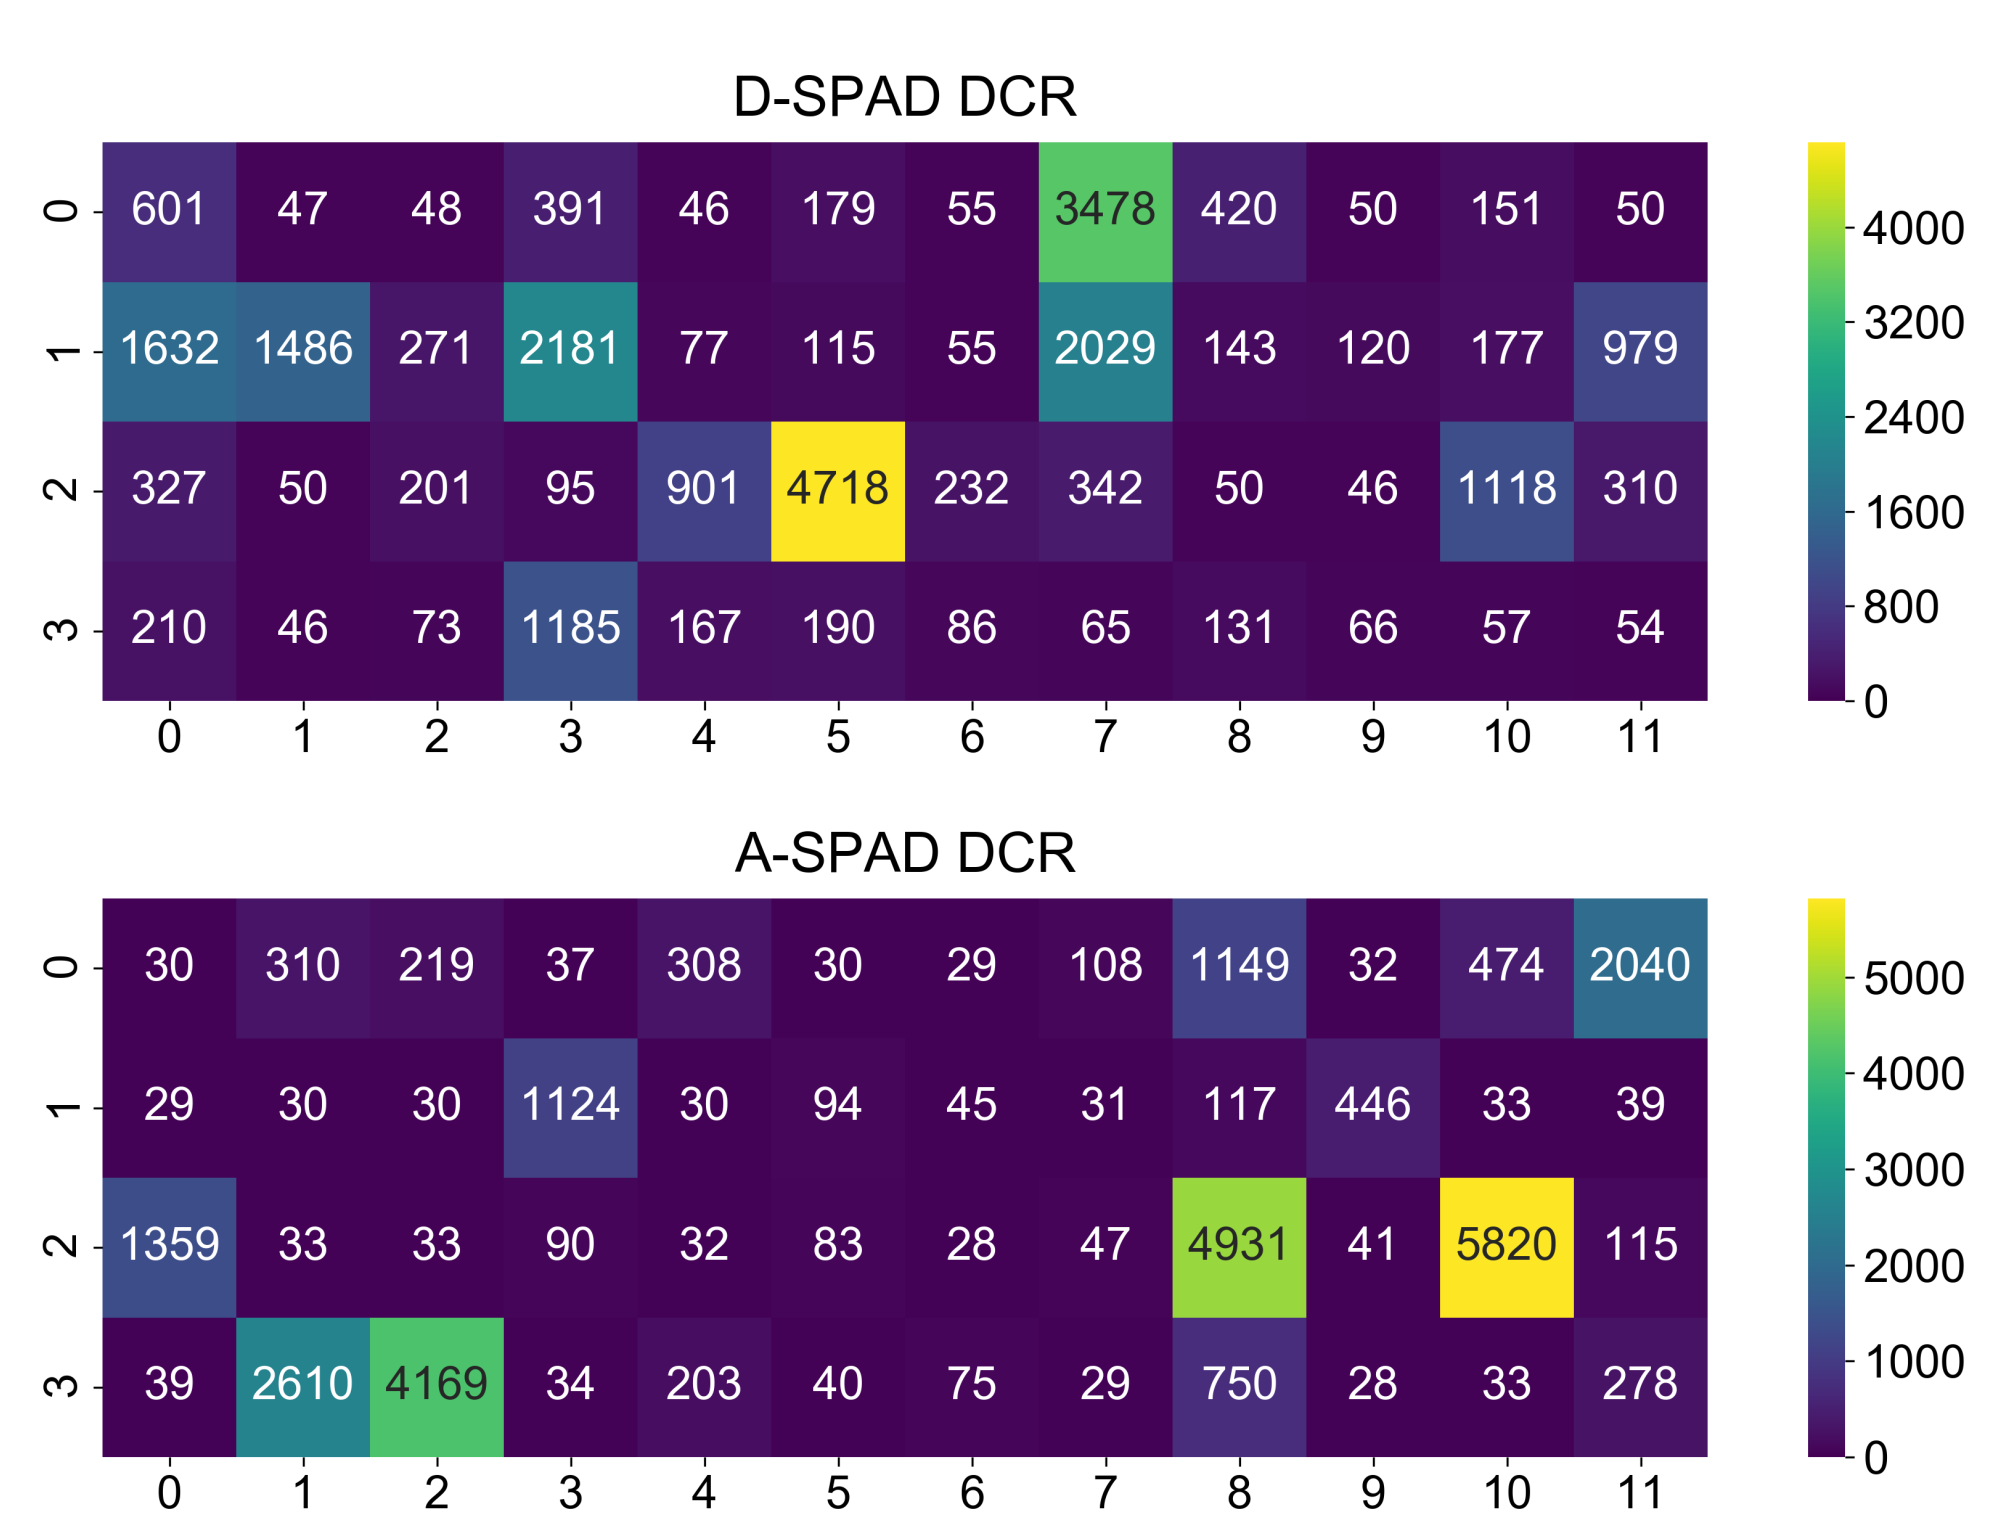
\includegraphics[width=\columnwidth]{figures/DCR-comp}
    \caption{\label{fig:dcr} Heatmaps of DCRs for the 12x4
    D- and A-SPAD arrays used in the  48-spot PAX setup.
    DCR values in counts per second (cps) are indicated in each pixel.
    More details and data can be found in the
    \href{http://nbviewer.jupyter.org/github/tritemio/48-spot-smFRET-PAX-analysis/blob/master/DCR\%20plots.ipynb}{DCR plots} analysis notebook.
}
\end{figure}

\subsection{48-spot pattern}
\label{sec:48spot-pattern}

The 48 excitation spots are generated independently for each wavelength by
phase modulation of the incoming laser wavefront, as previously described
in~\onlinecite{colyer_high-throughput_2010,ingargiola_multispot_2017}. The
phase modulation operates in direct space rather than Fourier space and
implements the phase profile of a Fresnel lenslet array.
Similar direct-space modulation using a different
spatial arrangement of the phase pattern on the LCOS-SLM have also been demonstrated 
for multi-confocal fluorescence correlation spectroscopy
(FCS)~\cite{kloster-landsberg_cellular_2012}.

Fig.~\ref{fig:patternfit} shows the emission pattern from a high-concentration dye sample
upon green (Panel A) and red (Panel B) laser excitation, as 
seen by a camera mounted on the microscope side-port. 
The two patterns are aligned to maximize overlap of each of the 48 spots.
Overlap of the two wavelengths and centering with respect to
the optical axis is assessed by 2D Gaussian fitting of each individual spot as reported in Panel C.
Full details on the alignment procedure and pattern assessment
can be found in Appendix~\ref{sec:lcos}.

\begin{figure}
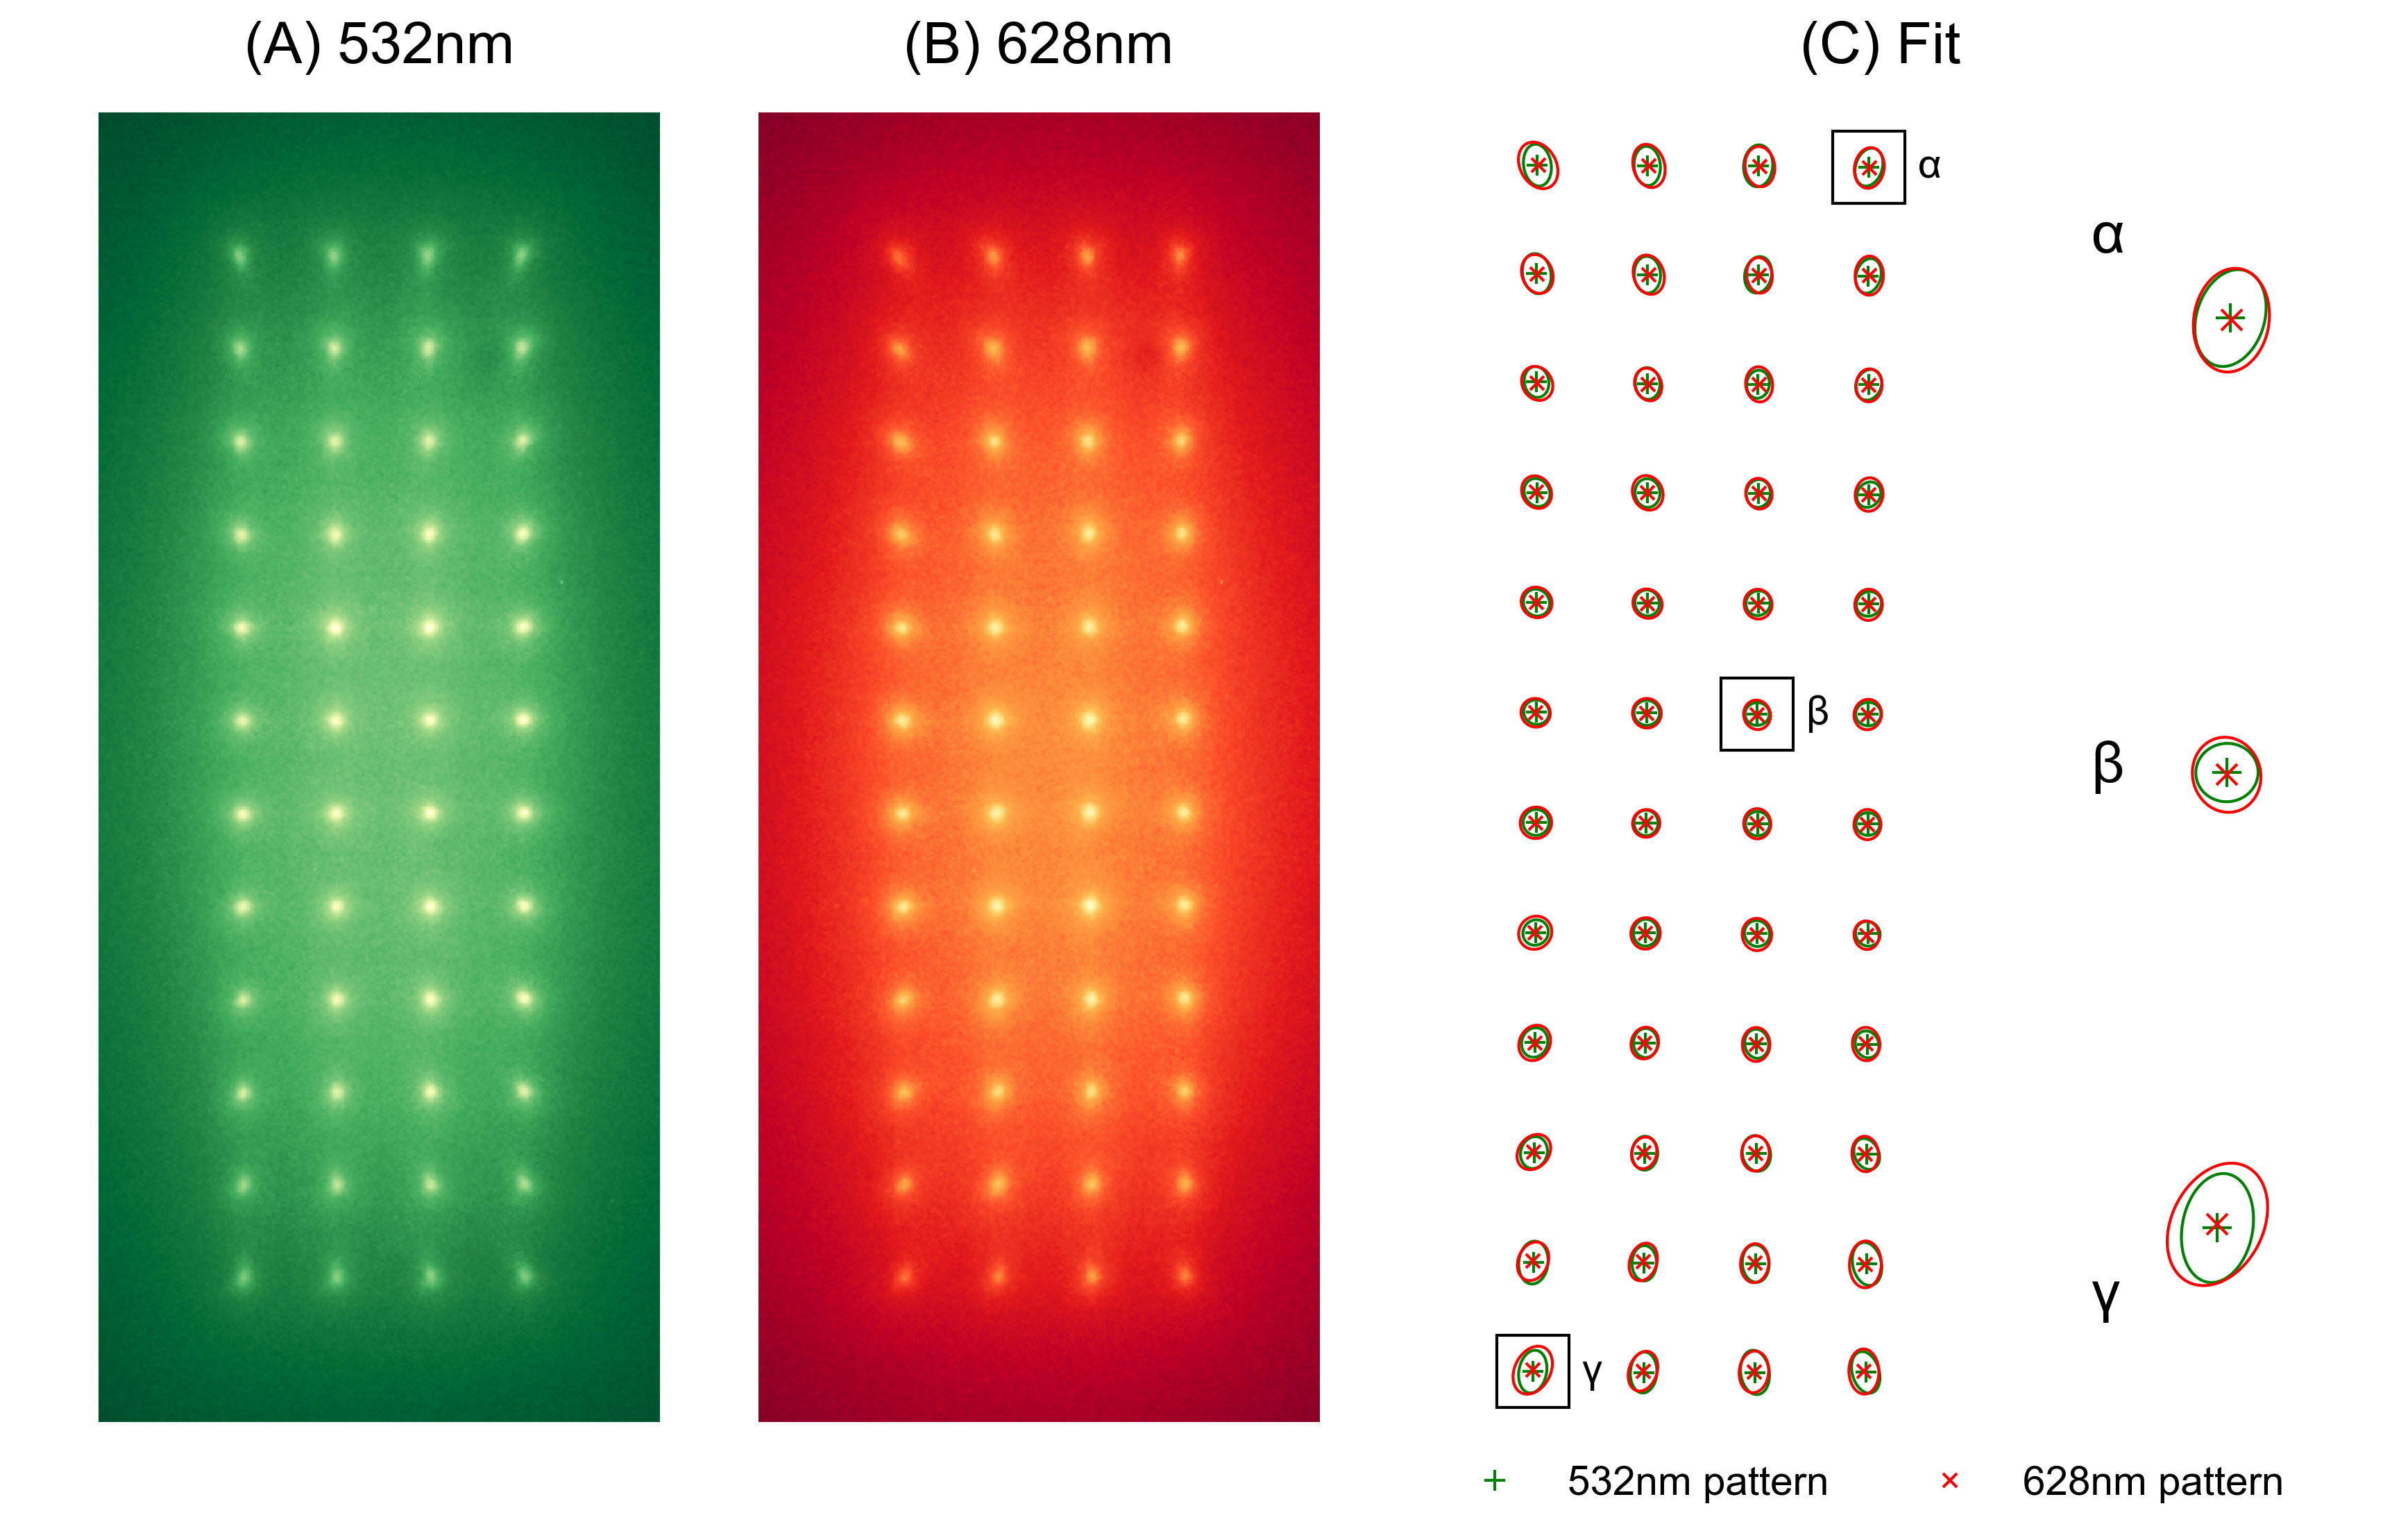
\includegraphics[width=\columnwidth]{figures/2017-04-28_conf9_G_conf14_R_green_red_pattern_and_fit}
    \caption{{\label{fig:patternfit}
    The 12x4 multispot pattern for green (A) and red (B)
    excitation and Gaussian fit of the spots (C). The pattern is acquired by
    a camera mounted on the microscope side port (see Fig.~\ref{fig:setup}) using a
    solution of ATTO550 and ATTO647N dyes at high concentration ($\sim$100~nM).
    Fluorescent images obtained upon 532~nm or 628~nm laser excitation were
    acquired separately and are reported in green and red intensity levels
    in panels (A) and (B), respectively. Scale bars are 5~{\micron}.
    To assess the alignment,
    each spot in the two images is fitted with a 2D Gaussian function. Panel
    (C) reports an overlay of the fitted peak positions and a
    contour of the Gaussian waist for 532~nm (\emph{green}) and 628~nm
    (\emph{red}) images. A closer look of 3 representative spots is reported on
    the right. The elliptical shape and tilt of the Gaussian is
    due to geometrical aberrations.
    More details can be found in the
    \href{http://nbviewer.jupyter.org/github/tritemio/48-spot-smFRET-PAX-analysis/blob/master/alignment/2017-04-28/pattern_profiling/LCOS\%20pattern\%20fitting-conf9\_G\_conf14\_R\_4x12\_slits.ipynb}{LCOS pattern fitting-conf9\_G\_conf14\_R\_4x12\_slits} notebook.
    }}
\end{figure}

\section{smFRET measurements}
\label{sec:smfret-meas}

\subsection{Analysis}
\label{sec:analysis}

Single-molecule measurements were performed with 40 base-pair (bp)
double-stranded DNA (dsDNA) molecules labeled with ATTO550 (D) and
ATTO647N (A) dyes (ATTOTEC GmbH, Heidelberg, Germany)
attached to different DNA bases, yielding different inter-dye distances.

D-A separation of 12~bp and 22~bp were used in these experiments,
as they cover the typical range of distances that can be accurately measured
with smFRET using this dye pair.
Samples were diluted to single-molecule concentration ($\sim50$~pM) in TE50
(10~mM Tris pH 8.0, 1 mM EDTA, and 50~mM NaCl) or in ``transcription buffer'' 
(40 mM HEPES-NaOH pH 7, 50 mM KCl, 10 mM MgCl$_{2}$, 1 mM DTT, 1 mM MEA, 
BSA: 100~\textgreek{μ}g/ml)~\cite{lerner_backtracked_2016}.
Full details regarding the DNA samples are provided in
ref.~\cite{ingargiola_multispot_2017}.

We analyzed data using standard {\usalex} methods~\cite{lee_accurate_2005}
with modifications required for PAX\cite{doose_periodic_2007}.
The three analysis steps include:
(a) background estimation, (b) burst search and (c) burst selection.
Background estimation, which is needed to correct the burst counts
in the different photon streams, was performed over 10~s time windows
in order to account for possible background variations during the measurement. 
Burst searches were performed independently for each spot
using the sliding-window algorithm~\cite{fries_quantitative_1998}
and a constant-rate threshold for all spots~\cite{ingargiola_fretbursts:_2016}.
Burst selection is performed taking bursts with size larger than a specified threshold,
where burst size is either defined according to eq.~\ref{eq:burstsize}
or~\ref{eq:burstsize_paxe}. To isolate the FRET populations, we
additionally filter bursts with $A_{ex}A_{em}$ counts larger
than a second specified threshold. Full numerical details can be found in the relevant notebook
on GitHub at
\href{https://github.com/tritemio/48-spot-smFRET-PAX-analysis}{48-spot-smFRET-PAX-analysis}.


The main result of the {\usalex} and PAX analysis methods is a so-called E-S two-dimensional histogram, where each burst is represented by a
pair of values $(E, S)$ computed from the distinct photon stream
intensities (see Section~\ref{sec:EShist}).
$E$ in that histogram can represent either the FRET efficiency or, more commonly
the uncorrected FRET efficiency, known as proximity ratio, $E_{PR}$.
$E_{PR}$ is easier to compute than $E$
and provides a suitable approximation for identifying sub-populations.
However, while it is not the objective of this study, 
when the purpose is to extract D-A distances $E$ must be computed, 
requiring accurate estimation of all correction coefficients.
$S$, or ``stoichiometry ratio'', is a quantity computed with all photon stream intensities, which typically has a value $\sim0.5$ for
doubly-labeled, $\sim0$ for A-only, and $\sim1$ for D-only species.
D and A-only species regions in that histogram also include doubly-labeled molecules with one inactive
dye due to photo-blinking or bleaching. Unlike the corrected stoichiometry
ratio $S_{\gamma\beta}$ (eq.~\ref{eq:Sgb}), the uncorrected ratio $S$
(eq.~\ref{eq:S}) can exhibit a dependence on $E$ and for doubly-labeled
molecules is not necessarily centered about 0.5.
The use of the $(E, S)$ pair (corrected or uncorrected)
allows separation of singly and doubly-labeled species and
distinguishing FRET sub-populations within the doubly-labeled population.
Full definitions of $E$ and $S$ as well as comparisons between ALEX and PAX
variants are reported in Appendix~\ref{sec:alex_pax}.

In this paper, we report proximity ratios $E_{PR}$ computed according to
eq.~\ref{eq:Epr}, and a ``modified stoichiometry ratio'' $S_u$ defined
in eq.~\ref{eq:Su}. $S_u$ is a variant of the classical
PAX stoichiometry ratio\cite{doose_periodic_2007}, which reduces the effect
of shot noise and improves the separability of D-only and FRET populations.
More details on $S_u$ can be found in Appendix~\ref{sec:Su}.
Note that throughout this work, the results of the two leftmost
spots in the second row are missing because of an active quenching circuit
(AQC) failure in the D-SPAD array.

\subsection{Peak photon rate}
\label{sec:peak-phrate}

\begin{figure*}
    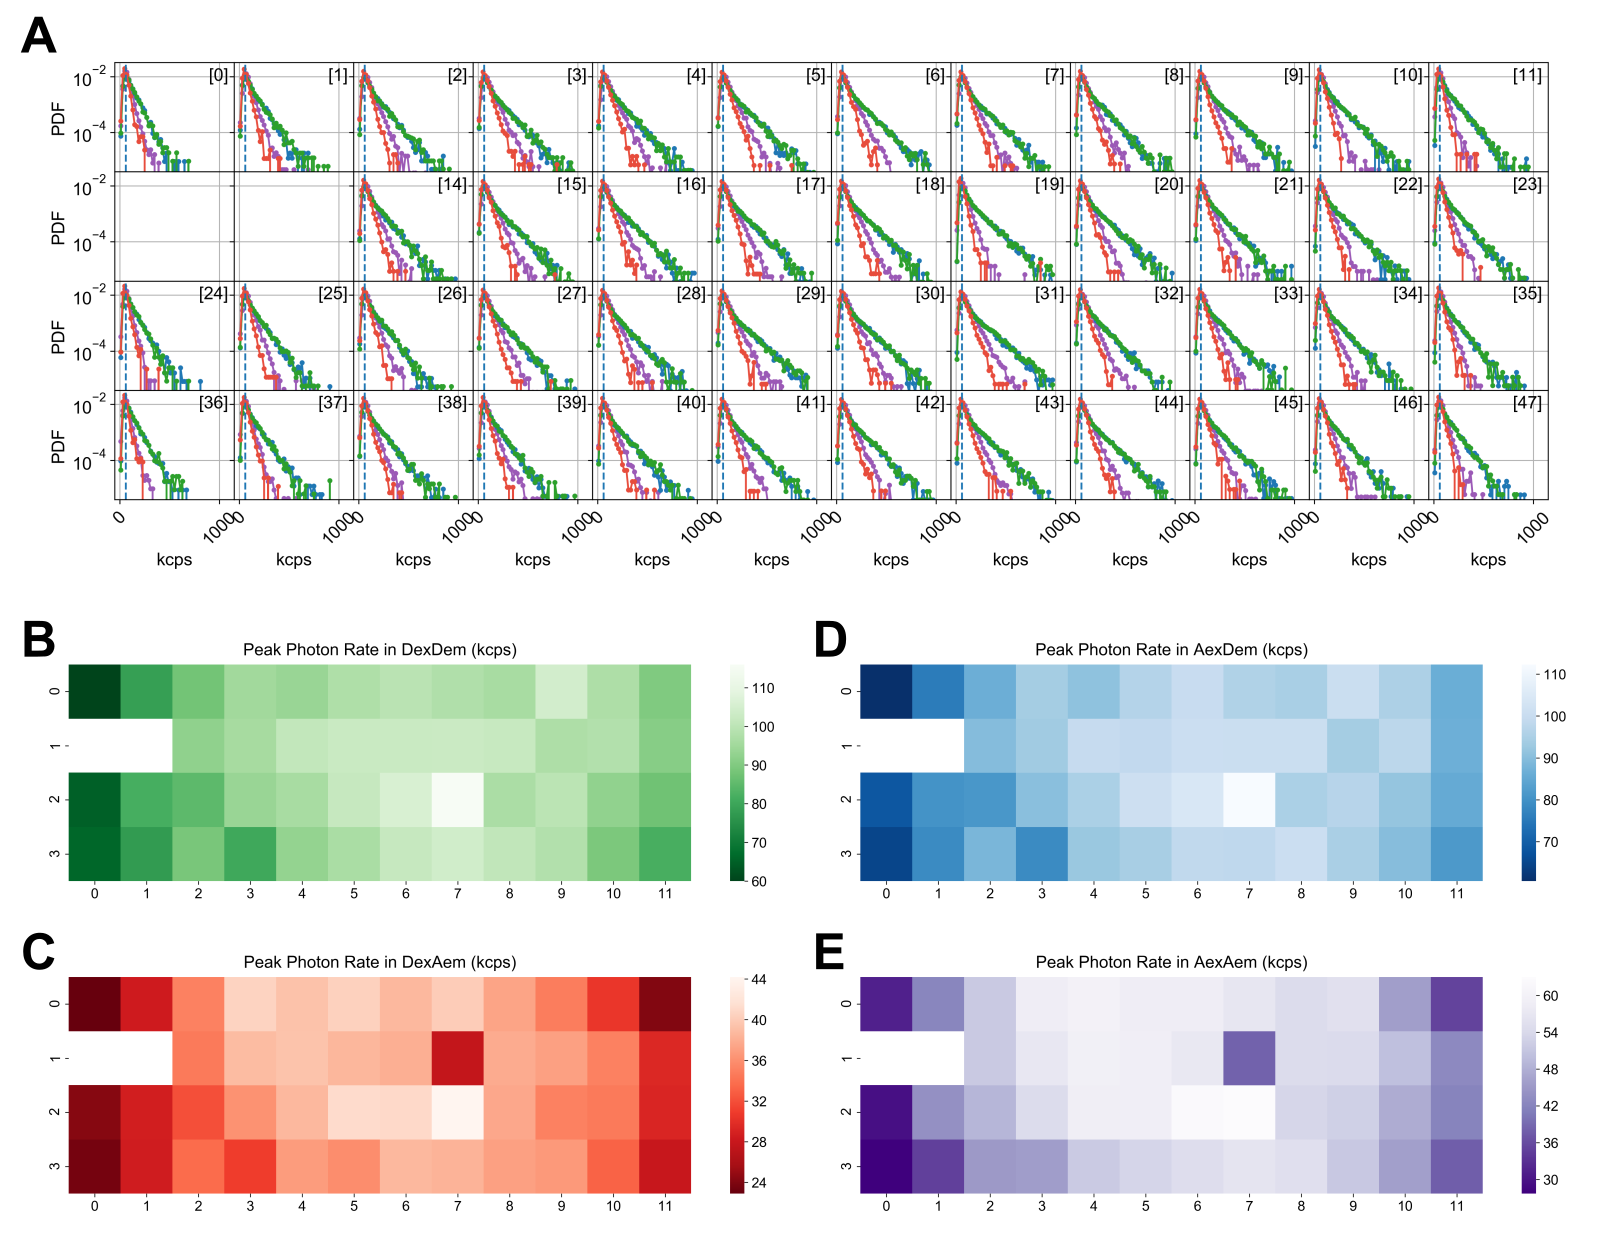
\includegraphics[width=\textwidth]{{figures/phrates_composite}}
    \caption{{\label{fig:phrates48_comp}
    Peak burst photon rates in each of the 48 spots for a dsDNA sample with a
    12~bp D-A separation. The output laser powers measured before any optics
    were set to 200~mW and 400~mW for the D- and A-laser respectively.
    A: Full distribution of peak photon rates. B-E: Mean of the peak photon
    rate distribution in different photon streams.
    Two lateral spots in the second row exhibit no signal because of
    two malfunctioning pixels in the D-SPAD array.
    Colors correspond to different photon streams.
    Green: $D_{ex}D_{em}$, red: $D_{ex}A_{em}$, light blue: $DA_{ex}D_{em}$,
    purple: $DA_{ex}A_{em}$. For more details see the
    \href{http://nbviewer.jupyter.org/github/tritemio/48-spot-smFRET-PAX-analysis/blob/master/smFRET-PAX\_single\_pop-2017-05-23\_08\_12d.ipynb}{smFRET-PAX\_single\_pop-2017-05-23\_08\_12d} notebook.
    }}
\end{figure*}

\begin{figure}
    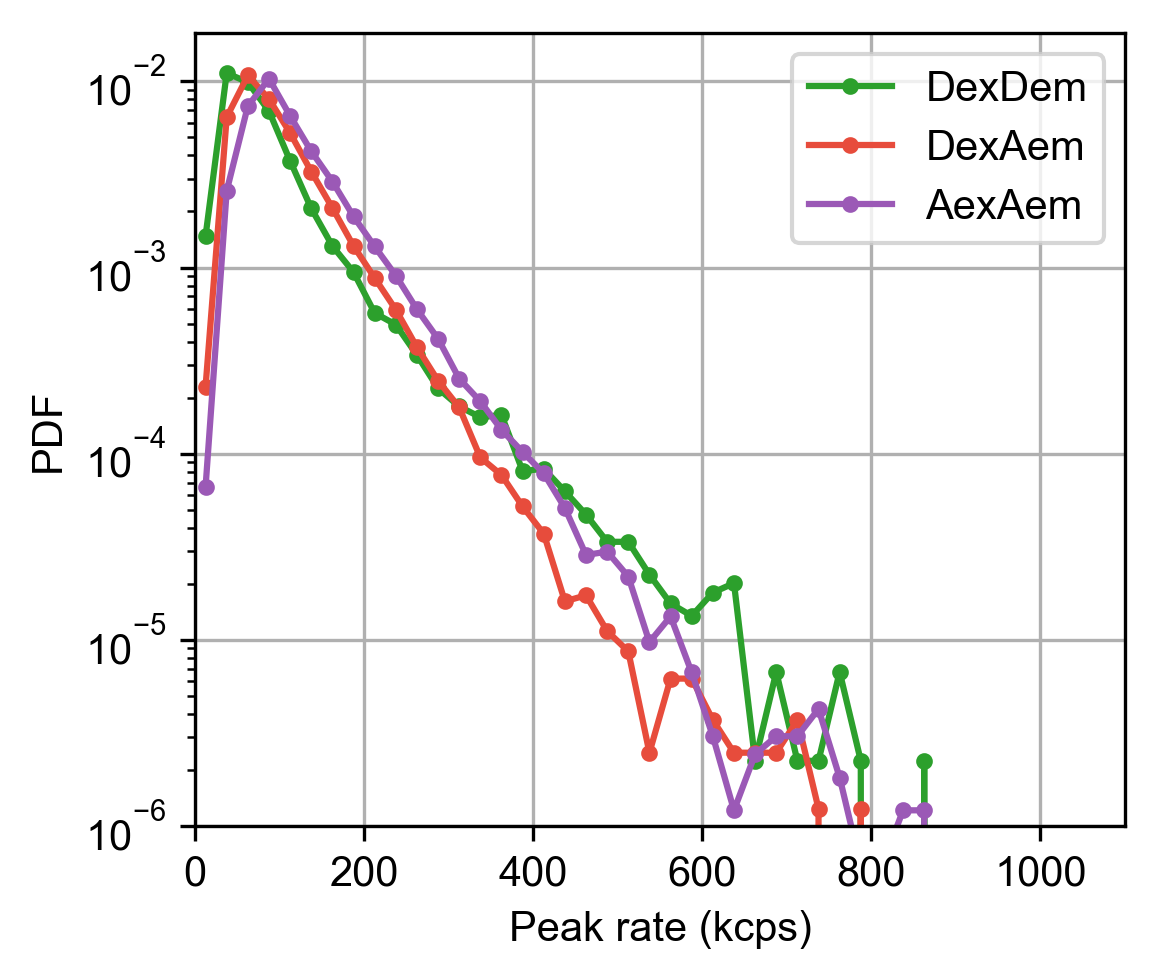
\includegraphics[width=0.7\columnwidth]{figures/2017-06-02_002_12d_usALEX_peak_phrate}
    \caption{{\label{fig:phrates_usalex}
    Distribution of peak photon rates in a single-spot {\usalex} measurement
    of the same dsDNA with a 12~bp D-A separation used in 48-spot
    measurements (Fig.~\ref{fig:phrates48_comp}). Average laser powers
    entering the microscope after AOM alternation were 190~\textgreek{μ}W and
    80~\textgreek{μ}W.
    Colors correspond to different photon streams.
    Green: $D_{ex}D_{em}$, red: $D_{ex}A_{em}$, light blue: $DA_{ex}D_{em}$,
    purple: $DA_{ex}A_{em}$.
    For more details see the notebook
    \href{http://nbviewer.jupyter.org/github/tritemio/48-spot-smFRET-PAX-analysis/blob/master/us-ALEX\_analysis-2017-06-11\_000\_12d.ipynb}{us-ALEX\_analysis-2017-06-11\_000\_12d}.
    }}
\end{figure}

The peak photon rate reached in each burst reports on the peak PSF
intensity~\cite{ingargiola_multispot_2017}.
Fig.~\ref{fig:phrates48_comp}A shows the background-corrected
peak photon rate distributions with their characteristic exponential tails.
Fig.~\ref{fig:phrates48_comp}B-E show, for different
photon streams, heatmaps of the peak photon rate mean values,
\textit{i.e.} the decay constant of the exponential tail.
Due to the Gaussian profile of the excitation beam and to geometric
aberrations, the lateral pixels receive a lower signal intensity than
the central pixels. As a result, the peak photon rate decreases and fewer
single-molecule bursts are detected in the lateral spots.
Despite this decrease in excitation intensity, the positions of the
$E_{PR}$ and $S$ peaks remains quite uniform across the spots
(see Fig.~\ref{fig:alexhist48fret12d} and~\ref{fig:fretfit48vsmean}).
An exception can be seen in Fig.~\ref{fig:phrates48_comp}C,E,
where the pixel at position (1, 7) in the A-SPAD array
detects fewer photons than its neighbors, an effect tentatively ascribed to a lower PDE
of that pixel possibly due to a lower applied overvoltage.
For this spot (19), we observe a noticeable bias in $E_{PR}$ and $S$
quantities
(see Fig.~\ref{fig:alexhist48fret12d} and~\ref{fig:fretfit48vsmean}).

By comparison, Fig.~\ref{fig:phrates_usalex} shows the distribution
of peak photon rates obtained with the {\usalex} setup.
The absolute power delivered in each spot in the multi-spot setup is
difficult to measure.
Therefore, we determined an optimal D-laser power (200~mW at laser
output) so that the peak photon rate distribution in the central spots
was comparable to the single-spot peak photon rate (190~\textgreek{μ}W
measured before the objective).
The A-laser power was set to 400~mW (laser output before the AOM),
as a trade-off between the need to compensate for the lower PDE in the
A-channel while limiting sample photo-bleaching and
thermal instabilities.

Comparing Figs.~\ref{fig:phrates48_comp}A and~\ref{fig:phrates_usalex}
it is clear that reduced sensitivity in the A-SPAD array results in lower peak
photon rates in the $D_{ex}A_{em}$ (red) and $DA_{ex}A_{em}$ (purple) streams
in the 48-spot setup. The sensitivity of the A-channel causes a shift in
the $E_{PR}$ and $S$ peak positions as discussed in the next Section.


\subsection{E-S histograms}
\label{sec:EShist}

\begin{figure*}
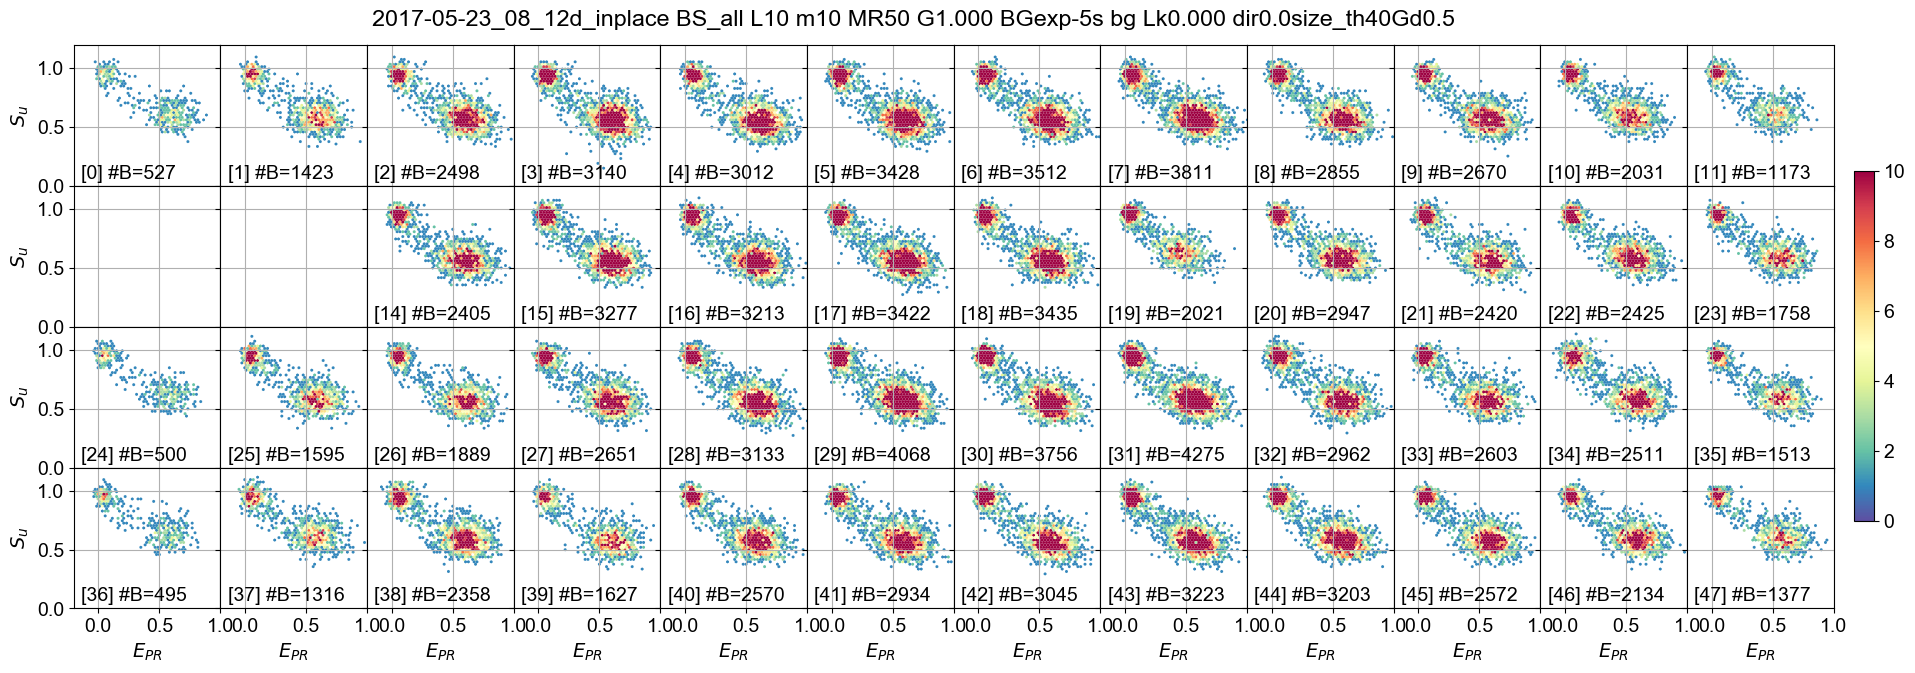
\includegraphics[width=\textwidth]{figures/2017-05-23_08_12d_48spot_alex_hist_Su_all-bursts}
\caption{{\label{fig:alexhist48all12d} $E_{PR}$ versus $S_u$
histograms in the different spots for the dsDNA sample with a 12~bp D-A separation.
Two subpopulations are visible: D-only (approximately $E_{PR}=0$,
$S_u=1$) and FRET population (approximately $E_{PR}=0.6$,
$S_u=0.6$). Burst search was performed using all photons with a 
constant threshold (50~kcps). Burst selection was performed
on the total burst size after background correction, using a threshold of
40 photons. The legend in each subplot reports the spot number in brackets and number of bursts (\#B).%
For more details see the
\href{http://nbviewer.jupyter.org/github/tritemio/48-spot-smFRET-PAX-analysis/blob/master/smFRET-PAX\_single\_pop-2017-05-23\_08\_12d.ipynb}{smFRET-PAX\_single\_pop-2017-05-23\_08\_12d} notebook.
}}
\end{figure*}

\begin{figure*}
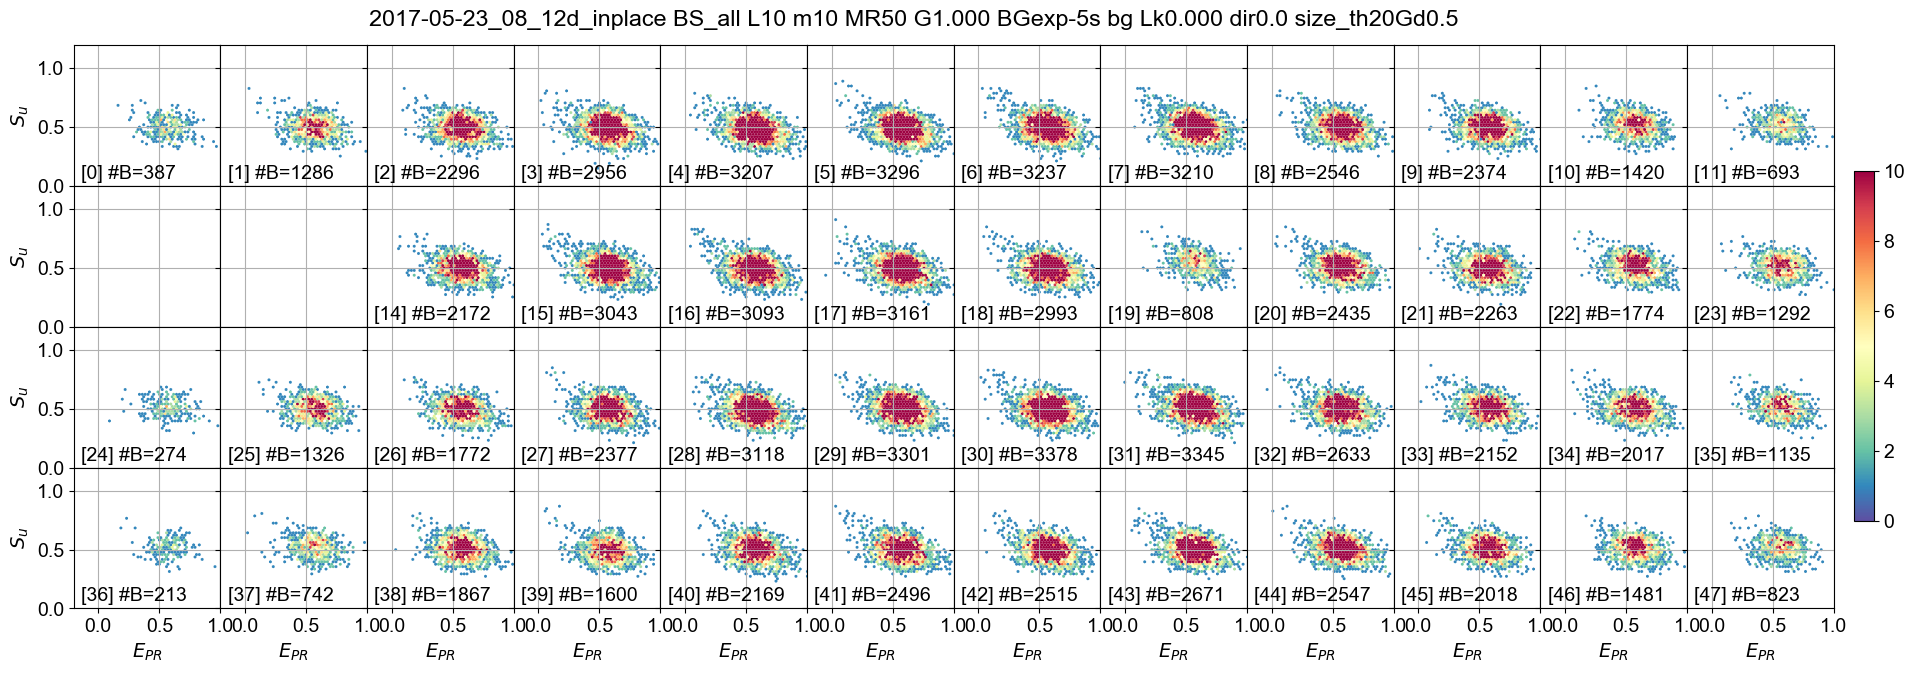
\includegraphics[width=\textwidth]{figures/2017-05-23_08_12d_48spot_alex_hist_Su_naa_AND_size_selection}
\caption{{\label{fig:alexhist48fret12d} $E_{PR}$ versus $S_u$
histograms in the different spots for the dsDNA sample with a 12~bp D-A separation.
Data analysis and
burst search are identical to figure~\ref{fig:alexhist48all12d}, while
burst selection is tailored to select only the FRET population: a burst is
selected if the number of counts in the $D_{ex}A_{em}$ and $DA_{ex}A_{em}$
streams are both larger than 20. The legend in each subplot
reports spot number in brackets and number of bursts (\#B).%
For more details see the
\href{http://nbviewer.jupyter.org/github/tritemio/48-spot-smFRET-PAX-analysis/blob/master/smFRET-PAX\_single\_pop-2017-05-23\_08\_12d.ipynb}{smFRET-PAX\_single\_pop-2017-05-23\_08\_12d} notebook.
}}
\end{figure*}

\begin{figure}
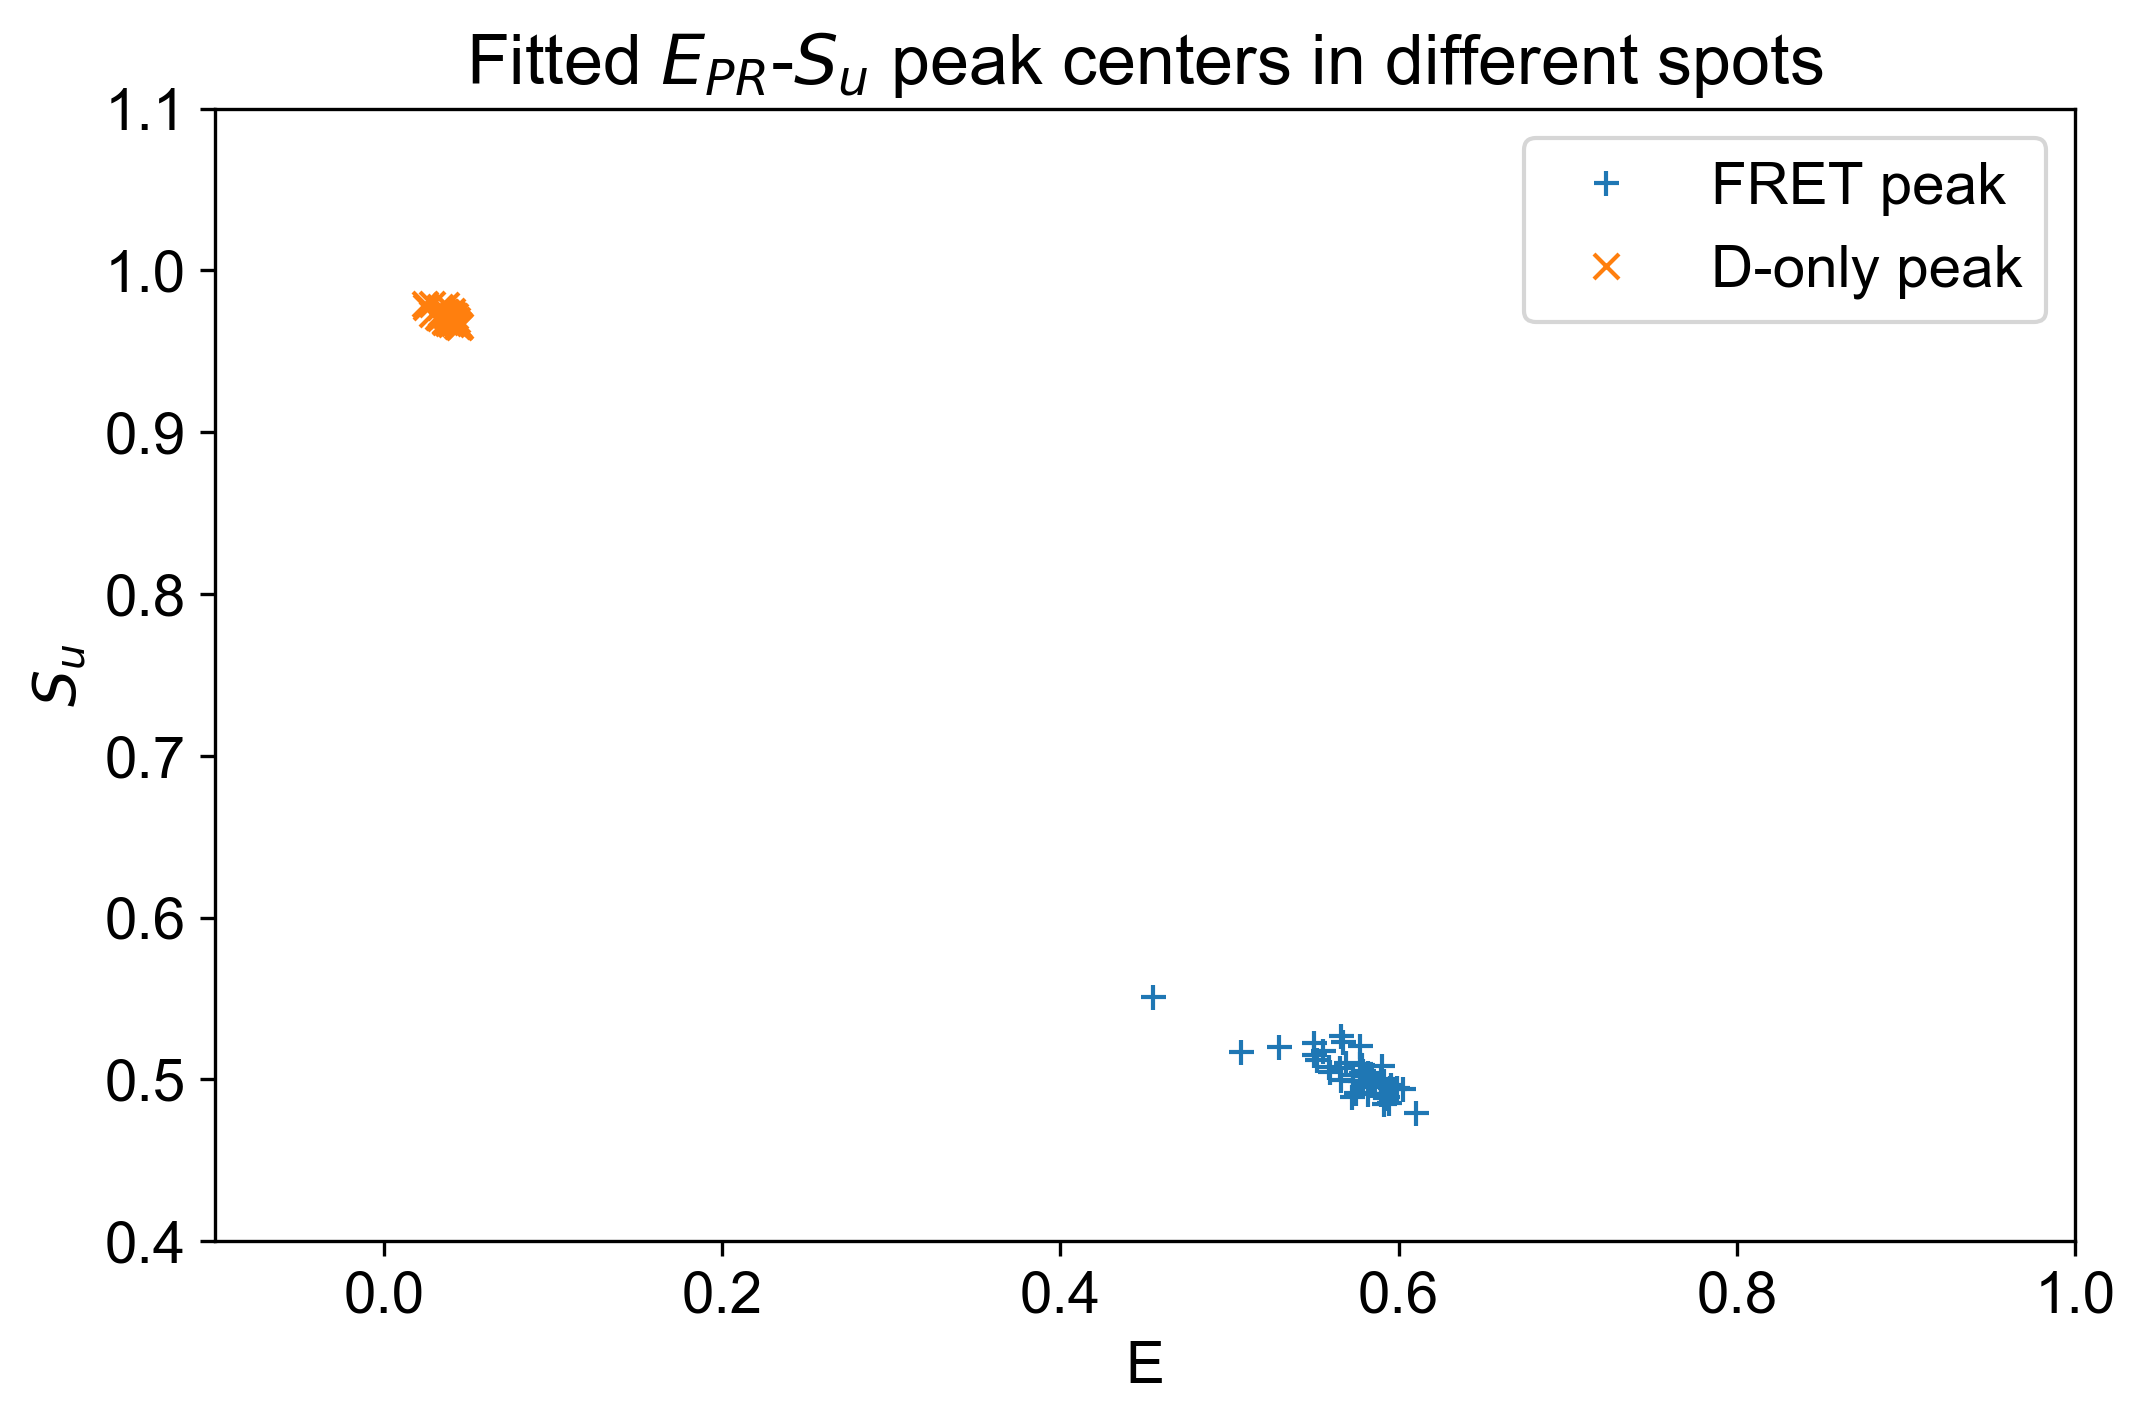
\includegraphics[width=0.9\columnwidth]{figures/2017-05-23_08_12d_FRET_vs_DO_fitted_Epr-Su_peak_position}
\caption{\label{fig:fittedFRETscatter}
Scatter plot of the fitted $E_{PR}$, $S_u$ peak
position in the different spots for the D-only (\emph{orange cross})
and FRET populations (\emph{blue plus}). Values were obtained by Gaussian
fit of the 1-D histogram of $E_{PR}$ and $S_u$ after a bursts selection
that isolated D-only and FRET populations, respectively.
For more details see the
\href{http://nbviewer.jupyter.org/github/tritemio/48-spot-smFRET-PAX-analysis/blob/master/smFRET-PAX\_single\_pop-2017-05-23\_08\_12d.ipynb}{smFRET-PAX\_single\_pop-2017-05-23\_08\_12d} notebook.
}
\end{figure}

\begin{figure*}
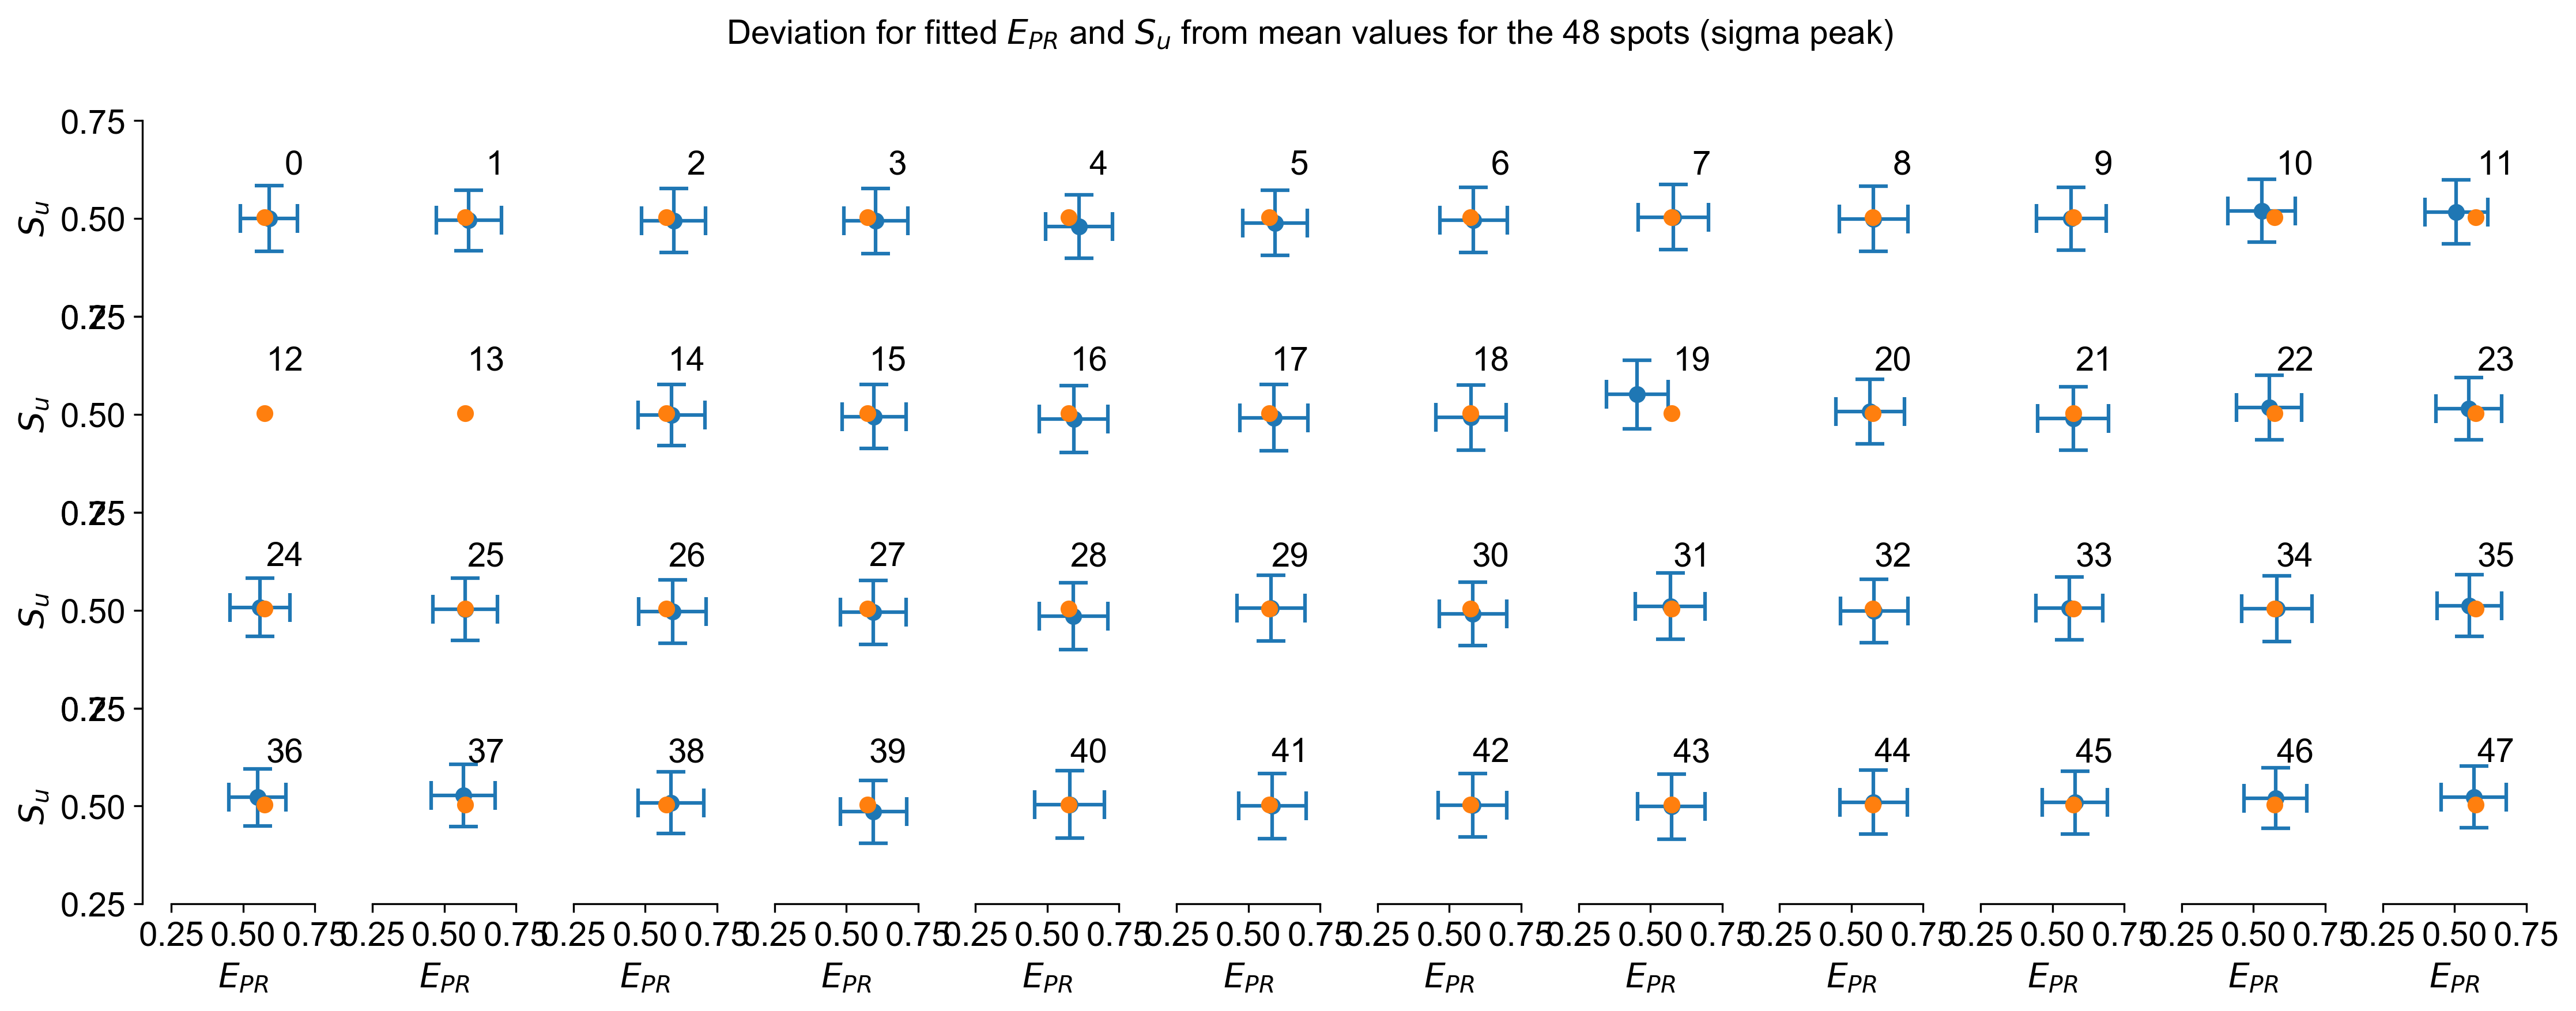
\includegraphics[width=\textwidth]{figures/2017-05-23_08_12d_48-spot_Epr-Su_peak_position_deviation_from_mean}
\caption{{\label{fig:fretfit48vsmean} Fitted FRET peak position ($E_{PR}, S_u$,
\emph{blue dots}) and $\pm 1 \sigma $ of the fitted Gaussian
(\emph{blue error bars}) for the 46 active spots. As a reference, the mean
$E_{PR}, S_u$ across all 46 spots (\emph{orange dot}) is reported
in each subplot. The spot number is indicated in the top right corner of
each subplot.%
For more details see the
\href{http://nbviewer.jupyter.org/github/tritemio/48-spot-smFRET-PAX-analysis/blob/master/smFRET-PAX\_single\_pop-2017-05-23\_08\_12d.ipynb}{smFRET-PAX\_single\_pop-2017-05-23\_08\_12d} notebook.
}}
\end{figure*}


Fig.~\ref{fig:alexhist48all12d} shows E-S histograms for the
dsDNA sample with a 12~bp D-A separation,
obtained after the burst search and size selection
described in Section~\ref{sec:analysis}.

The D-only and FRET populations, top left corner
and center respectively in the E-S histogram, are clearly distinguishable in all spots.
Moreover, as shown in Fig.~\ref{fig:alexhist48fret12d}, 
the FRET population(s) are easily isolated by applying a second burst
selection using a minimum threshold on the $DA_{ex}A_{em}$ counts.
A second example of such a selection is shown in Fig.~\ref{fig:ES48mix-fret}.
Separation of FRET species from singly-labeled species is the primary advantage
of dual laser excitation~\cite{li_ultrasensitive_2003,kapanidis_fluorescence-aided_2004}.

Even without any calibration, the spread across different spots
is limited and does not affect the ability to distinguish subpopulations.
This is evident in Fig.~\ref{fig:fittedFRETscatter}, which shows the
$E_{PR}$ and $S_u$ peak center position in different spots for
both D-only and FRET populations.
Fig.~\ref{fig:fretfit48vsmean} shows the center and $\pm1\,\sigma$
range from Gaussian fits of $E_{PR}$ and $S_u$ histograms
of the FRET population (blue dot and error-bar).
The orange dot is the mean center peak position of the FRET population
across all spots. For most spots, the
deviation of the peak position is well below the $\pm1\,\sigma$
range, with the exception of spot 19, where
the lower A-pixel PDE causes a larger deviation.
Note that Fig.~\ref{fig:fittedFRETscatter} and~\ref{fig:fretfit48vsmean}
present results without calibration, thus showcasing the minimum
performance of the system.
It is possible to virtually eliminate spot-to-spot variations
of the E-S peak position during post-processing by applying
a spot-specific calibration, as briefly
described in the next Section (details in Appendix~\ref{sec:perchcorr}).
As an additional example, the E-S histogram for a low FRET dsDNA
(22~bp D-A separation) is reported in Fig.~\ref{fig:alexhist48all22d},
Appendix~\ref{sec:moredata}.

\subsection{Pooling data from all spots}
\label{sec:alexpax-comp}

\begin{figure}
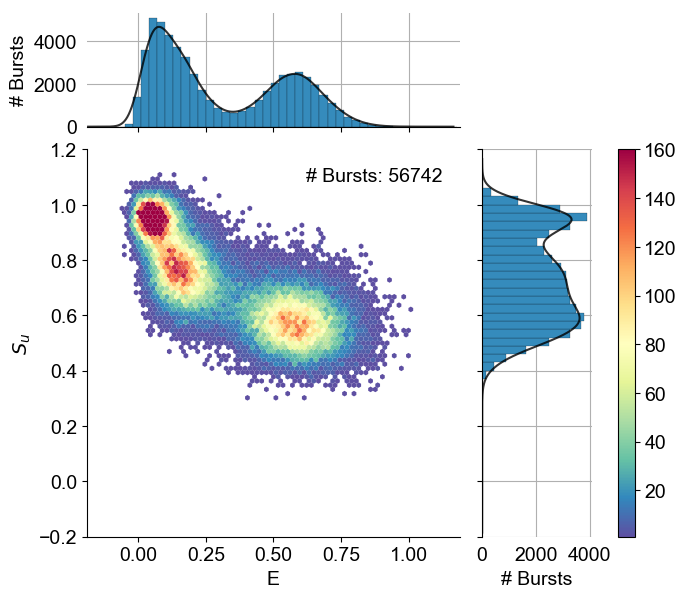
\includegraphics[width=\columnwidth]{figures/2017-07-11_06_12d_22d_ES-hist-collapsed-all-pops}
\caption{\label{fig:ES48mix-all}
48-spot PAX measurement of a mixture of two dsDNA constructs with 12 and
22~bp D-A separation (sample details in~\ref{sec:analysis}).
Burst search was performed on all channels
using a constant-rate threshold of 50~kcps.
Burst were selected based on their total size with the criterion $\Lambda_{\gamma,PAX} > 80$,
using $\gamma = 0.5$ (see eq.~\ref{eq:burstsize_paxe}).
The E-S histogram was built by pooling data from all spots, without 
spot-specific correction.
For more details, see the 
\href{http://nbviewer.jupyter.org/github/tritemio/48-spot-smFRET-PAX-analysis/blob/master/smFRET-PAX\_single\_pop-2017-07-11\_12d-22d-mixture.ipynb}{smFRET-PAX\_single\_pop-2017-07-11\_12d-22d-mixture} notebook.
}
\end{figure}

\begin{figure}
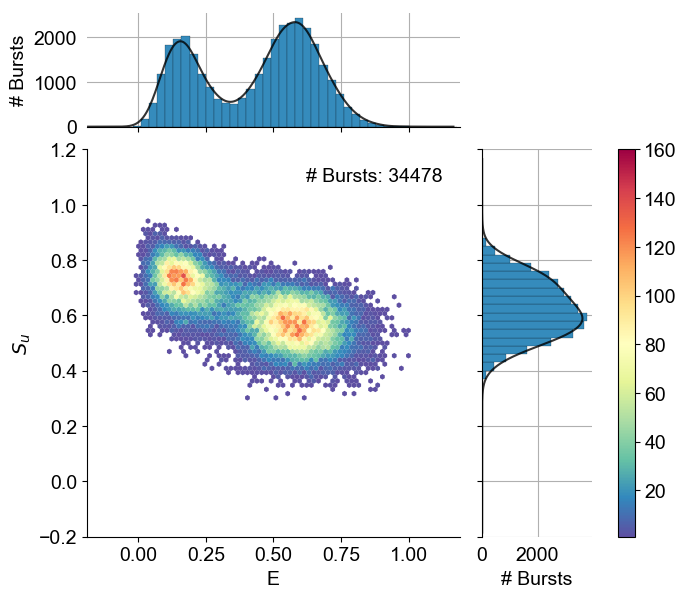
\includegraphics[width=\columnwidth]{figures/2017-07-11_06_12d_22d_ES-hist-collapsed-FRET-pops}
\caption{\label{fig:ES48mix-fret}
48-spot PAX E-S histograms of the same measurement of
Fig.~\ref{fig:ES48mix-all}. Additional filtering of the D-only population
was performed using the criterion $F_{D_{ex}DA_{em}} > 25$
(see Appendix~\ref{sec:alex_pax}).
The E-S histogram was built by pooling data from all spots without 
spot-specific correction.
For more details, see the
\href{http://nbviewer.jupyter.org/github/tritemio/48-spot-smFRET-PAX-analysis/blob/master/smFRET-PAX\_single\_pop-2017-07-11\_12d-22d-mixture.ipynb}{smFRET-PAX\_single\_pop-2017-07-11\_12d-22d-mixture} notebook.
}
\end{figure}

The final step of multispot analysis consists in merging data from all
spots in order to increase the effective data accumulation rate.
Non-uniformities between different spots can be accounted for by applying a two-step 
correction, in which each correction factor $\gamma$ and $\beta$
(Eq.~\ref{eq:gamma} and~\ref{eq:beta}) is decomposed into a product of two factors 
applied successively: an average correction factor computed over all spots and a 
spot-specific relative correction.
The spot-specific correction of $\gamma$ and $\beta$ can be easily computed
from a measurement of a static FRET sample
(details in Appendix~\ref{sec:perchcorr}).
For simplicity and due to the good uniformity among spots, we do not apply any 
spot-specific corrections in this work.

Fig.~\ref{fig:ES48mix-all} shows the cumulated E-S histograms of a mixture
of two dsDNA constructs with D-A separation of 12 and
22~bp (see Section~\ref{sec:analysis}),
resulting in mean $E_{PR}$ of $\sim0.6$ and $\sim0.15$ respectively.
A significant D-only population is visible as a peak close to $E_{PR}=0.05$,
$S_u=1$. Due to the relatively low PDE
of the acceptor channel (see Section~\ref{sec:detectors}), the separation
of D-only and FRET populations could be problematic in principle.
As previously shown (Fig.~\ref{fig:alexhist48fret12d}),
FRET populations can be selected by setting a threshold on 
background-corrected $DA_{ex}A_{em}$ counts.
Fig.~\ref{fig:ES48mix-fret} shows that this selection effectively
removes the large D-only peak, isolating the FRET populations
without significant loss of FRET bursts.
As an illustration of the high-throughput capabilities of our setup,
Fig.~\ref{fig:alex_mspot_5} and~\ref{fig:alex_sspot_5}
show an example from 5~s-long acquisition windows obtained with the same doubly-labeled
dsDNA sample droplet, successively using the single-spot {\usalex} and multispot
setups (the sample is the 12~bp D-A separation dsDNA described in 
Section~\ref{sec:analysis}).
In both cases, a constant rate-threshold (20 kcps) burst search was used, followed by 
burst selection based on $D_{ex}$ counts ($\Lambda > 80$).
The particular time windows illustrated in Fig.~\ref{fig:alex_mspot_5} 
and~\ref{fig:alex_sspot_5} shows a 37-fold difference in burst numbers between the two 
measurements ($40 \pm 11$-fold computed over all consecutive 5~s windows within the two 
5~min acquisitions), reasonably consistent with the 46-fold difference 
expected between the two setups, assuming that all experimental conditions are 
identical. The large standard deviation of the measured ratio reflects the naturally 
large variance of the burst rate (number of bursts per unit time) within any given 
measurement. Moreover, since the burst rate depends on a number of measurement and 
analysis parameters, the burst rate ratio should not be given excessive significance.
For instance, the lower power in the lateral spots of the multispot setup (see
Fig.~\ref{fig:patternfit}) will result in smaller bursts and
therefore less bursts surviving the selection. While the lower detection efficiency of 
the SPAD array in the red region of the spectrum (compared to the single-spot setup, 
see Section~\ref{sec:detectors}) reduces the acceptor signal in the multispot 
measurement, also resulting in smaller and fewer bursts above the size selection 
threshold, this potential source of differences was compensated by the use if 
$\gamma$-corrected burst sizes (eq.~\ref{eq:burstsize}).
Finally, differences in observation volumes between setups, as indicated by the 
slightly larger burst durations in the multispot measurement (suggesting larger 
volumes), will also translate in different detected burst rates. Despite these 
caveats, it is obvious that the multispot setup detects a much larger number of bursts 
than the  single-spot setup.

Comparison of Fig.~\ref{fig:alex_mspot_5} and~\ref{fig:alex_sspot_5} shows 
that a significant number of bursts (~1,000) can be obtained in only a few seconds 
of acquisition.
Such a high throughput is advantageous for stop-flow or equivalent, real-time kinetic 
measurements, where a reaction is triggered at time zero and the sample's evolution
monitored continuously afterward.
The measurement's temporal resolution, \textit{i.e.} the smallest usable time window 
(or time bin), depends inversely on the burst rate (as well as on the type of 
information to be extracted from  the data), based on number statistics.
In the simple case where the initial and final FRET states of a reaction are known, 
and the respective amount of each population is an appropriate reaction parameter, 
the number of burst in each subpopulation can be extracted from the FRET histogram 
with a relatively small number of bursts per time bin. The number of bursts collected 
in the experiment reported in Fig.~\ref{fig:alex_mspot_5} would definitely be 
compatible with an effective time resolution $\le5$~s.
To fully take advantage of such a temporal resolution, the experimental dead-time 
(duration  of the initial mixing step in the reaction) would need to be shorter, 
and may require an automated microfluidic system ($\ll$~1~s, by contrast with the 
manual mixing reported in the kinetic measurement of ref.~\cite{ingargiola_multispot_2017}, where a deadtime of at least 15-20~s was 
obtained).
Such a multispot system could also advantageously be used to perform rapid series of
measurements of the same sample in different conditions, or of different samples, for
high-throughput screening applications, among other possibilities.

\begin{figure}
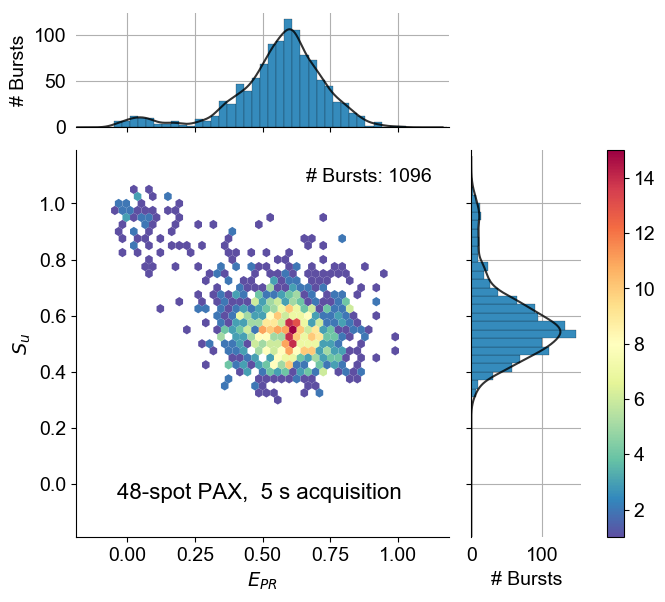
\includegraphics[width=\columnwidth]{figures/2017-08-03_03_12d_alex_jointplot_5s_Dex}
\caption{\label{fig:alex_mspot_5}
Multispot E-S histogram obtained from 5~s of acquisition by pooling bursts
from the 46 active spots.
For more details see the 
\href{http://nbviewer.jupyter.org/github/tritemio/48-spot-smFRET-PAX-analysis/blob/master/smFRET-PAX\_ALEX-PAX\_comparison\_2017-08-03\_03\_12d.ipynb}{smFRET-PAX\_ALEX-PAX\_comparison\_2017-08-03\_03\_12d} notebook.
}
\end{figure}

\begin{figure}
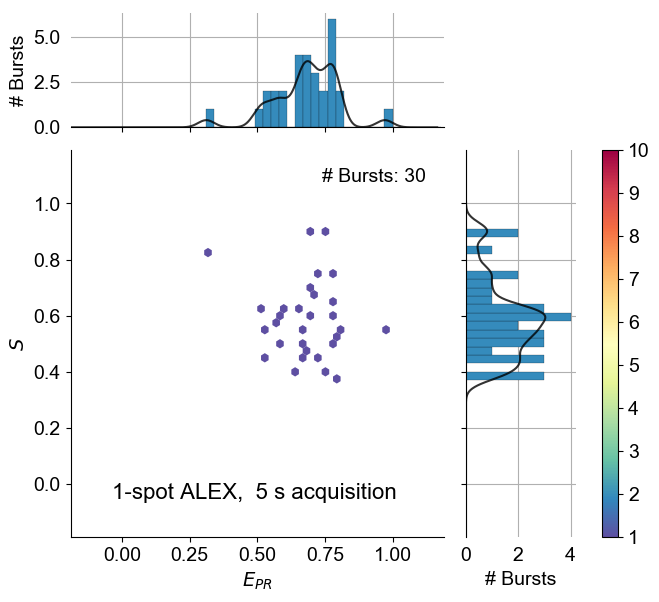
\includegraphics[width=\columnwidth]{figures/2017-08-03_007_12d_alex_jointplot_5s_Dex}
\caption{\label{fig:alex_sspot_5}
Single-spot E-S histogram obtained from 5~s of acquisition for the same
sample as in Fig.~\ref{fig:alex_mspot_5}.
For more details see the 
\href{http://nbviewer.jupyter.org/github/tritemio/48-spot-smFRET-PAX-analysis/blob/master/smFRET-PAX\_ALEX-PAX\_comparison\_2017-08-03\_03\_12d.ipynb}{smFRET-PAX\_ALEX-PAX\_comparison\_2017-08-03\_03\_12d} notebook.
}
\end{figure}

\section{Conclusion}
\label{sec:conclusion}
We have described a 48-spot, 2-laser excitation setup
designed for high-throughput smFRET assays.
Compared to our previous multispot setup~\cite{ingargiola_multispot_2017},
the number of spots was increased six-fold with a corresponding increase
in throughput.
While larger SPAD arrays have been demonstrated by other groups,
they are fabricated using standard high-voltage CMOS processes
resulting in poorer photon-counting performance than the custom technology
process employed here. Convincing applications for cell FCS and FLIM,
among others, have been published with these CMOS SPAD
arrays~\cite{colyer_ultra_2011,burri_65k_2014,buchholz_fpga_2012,kloster-landsberg_note:_2013,kufcsak_time-resolved_2017,kufcsak_time-resolved_2017},
(for a comprehensive review see~\onlinecite{bruschini_ten_2017})
but they still remain far from providing the sensitivity needed for
single-molecule applications.

Compared to our previous works~\cite{ingargiola_multispot_2017,ingargiola_16ch_2017},
a second alternating excitation laser was incorporated,
and the corresponding alignment hurdles were solved,
permitting sorting of single-molecules according to their
D-A stoichiometry. In particular, we have shown that the setup
allows identifying singly and doubly-labeled species over the full range
of FRET efficiencies, opening the door to a much wider range of assays
than was previously possible.

We presented a detailed description of the multispot setup and alignment
procedure, which incorporates a number of technical solutions of potential
interest for other applications.
We also illustrated the smFRET measurement capabilities of the new setup
using doubly-labeled dsDNA molecules as a proof of principle
demonstration of sub-population separations and high-throughput measurements.
Finally, we provided a comparison of its performance with a standard
single-spot (confocal) {\usalex} setup.
Applications of this new instrument to the study of the initial
stages of bacterial transcription and high-throughput diagnostics
will be explored in future work.

\begin{acknowledgments}
The authors thank Luca Miari for help in the initial stage of this project,
Mr. Yazan Alhadid and Dr. Eitan Lerner for help with single-molecule
sample preparation and Dr. Eitan Lerner for critical reading of the manuscript.
We thank Dr. Bentolila for the generous loan of a LCOS-SLM from the
Advanced Light Microscopy/Spectroscopy Shared Resource Facility at
the California NanoSystems Institute at UCLA.
Research reported in this publication was supported by the National Institute
of General Medical Sciences of the National Institutes of Health under
Award Number R01 GM095904 \& R01 GM069709, and by the National Science
Foundation under Award Number MCB 1244175.
The content is solely the responsibility of the authors and does not
necessarily represent the official views of the National Institutes of
Health or the National Science Foundation.
Conflict of interest statements: S. Weiss discloses intellectual
property used in the research reported here. M. Ghioni discloses equity in Micro Photon Devices S.r.l. (MPD). No resources or personnel from MPD were involved in this work.
The work at UCLA was conducted in Dr. Weiss's Laboratory.

\end{acknowledgments}


\appendix

\section{Detailed setup description}
\label{sec:setup}

The setup (Fig.~\ref{fig:setup}) comprises two excitation CW lasers emitting at
532~nm and 628~nm (2RU-VFL-Series, MPB Communications Inc., QC, Canada).
For each laser, a half-wave plate and polarizing beam splitter are used
for polarization and intensity control, as the polarization orientation
must be aligned along the direction required by the LCOS-SLM. The
628 nm laser beam passes through an AOM (P/N 48058
PCAOM, electronics: P/N 64048-80-.1-4CH-5M, Neos Technology, Melbourne,
FL) used for {\microsec} time-scale modulation. The 532~nm
laser is not modulated.
Each laser beam goes through a first beam expander (Keplerian
telescope, doublet lenses: 50~mm and 250~mm focal lengths). Two periscopes
bring the beams to a raised optical breadboard where an inverted microscope body
(X71, Olympus Corp., Waltham, MA) stands, its bottom port sitting
over a circular aperture in the breadboard. Beyond the periscope, each beam goes through a
second adjustable beam expander (3X, P/N 59-131, Edmund Optics Inc.).
The red laser beam is reflected off mirrors $M1_R$ and
$M2_R$ and phase-modulated by the ``red'' LCOS-SLM (P/N
X10468-07, Hamamatsu, Japan), before passing through the dichroic mirror
$D_{MIX}$. The green laser beam is reflected off $M3$, is
phase-modulated by the ``green'' LCOS-SLM (P/N X10468-01, Hamamatsu)
and combined with the red excitation via the dichroic mirror
$D_{MIX}$ (T550LPXR, Chroma Technology Corp, VT). Both
beams are recollimated by the $L_3$ lens (f = 250~mm,
AC508-250-A, Thorlabs) and focused into the sample by a high-NA
water immersion objective lens (UAPOPlan 60X, NA 1.2, Olympus) after being reflected off
the excitation dichroic mirror $DM_{EX}$ (Brightline
FF545/650-Di01, Semrock Inc., NY). The excitation pattern forms a
dual-color 12x4 array of spots in the sample, matching the geometry of
the two SPAD arrays. The fluorescence emission is collected by the same
objective lens, passes through the excitation dichroic
$DM_{EX}$ and is focused by the microscope's tube lens $L_2$ on either
the side or bottom port of the microscope. The side port is equipped with a
CMOS camera (Grasshopper3 GS3-U3-23S6M-C, FLIR Integrated Imaging
Solutions Inc., BC, Canada) used during alignment, while the bottom port
redirects the beams toward the SPAD array emission path. Here, a relay lens
$L4$ (f = 100~mm, AC254-100-A, Thorlabs) recollimates the
image and sends it to an emission dichroic mirror $D_{EM}$
(Brightline Di02-R635, Semrock), which splits the signal into donor
(D) and acceptor (A) spectral bands. The D signal goes through a band-pass
filter (Brightline FF01-582/75, Semrock) which removes residual 628~nm
laser leakage and helps suppress Raman scattering from the 532~nm
laser. Both D and A signals are refocused by lenses $L5_D$ /
$L5_A$ (f=150~mm, AC254-150-A, Thorlabs) on two 48-pixel
SPAD arrays\cite{gulinatti_48-pixel_2013} (denoted as D and A-SPAD in
the text).

Both SPAD arrays are mounted on 3-axis micro-positioners. Motion along the
X \& Y directions orthogonal to the optical axis  are software-controlled
via open-loop piezo-actuators
(P/N 8302; drivers: P/N 8752 \& 8753; Newport
Corporation, Irvine, CA). The third axis (Z) uses a manual actuator,
as requirements on the Z direction are much less stringent than
for the X \& Y directions. The D-SPAD array is mounted on an additional rotation stage
about the optical axis, which is used to match the relative orientation
of the SPAD arrays. Software for controlling the micro-positioners is
available in the
\href{https://github.com/multispot-software/picomotor}{picomotor} repository.

Each SPAD array module is equipped with an internal FPGA
(Xilinx Spartan 6, model SLX150), a humidity sensor, and a USB 2.0 connection.
The default FPGA firmware used in this work allows acquisition of low-resolution
(10-100~ms) time-binned counts via the USB connection, and is also used
for humidity monitoring. In addition, a standard SCSI connector
includes 48 independent outputs providing a pulse for every detected
photon in each pixel~\cite{gulinatti_48-pixel_2013}. The two SCSI ports are fed
through a custom adapter to an FPGA-based acquisition board (FPGA board:
PXI-7813R, PXI rack: PXI-1000B, National Instruments, Austin, TX) which
performs photon time-stamping with 12.5~ns resolution in parallel on the 96
channels (task implemented in LabVIEW using the LabVIEW FPGA Module,
code available \href{https://github.com/multispot-software/MultichannelTimestamper}{here}).
The FPGA board transfers data asynchronously to a host PC via an MXI-4 link
to a custom acquisition program written in LabVIEW (PXI rack board: PXI-8331;
PC board:PCI-8331, National Instruments). The
acquisition program also controls the red laser alternation using a
pulse generation board (PXI-6602, National Instruments) with a clock
synchronized to the time-stamping FPGA board through the PXI rack.

In addition to the aforementioned acquisition program, the host computer
runs a second LabVIEW program controlling the phase pattern on the
two LCOS-SLMs. During alignment, the acquisition program communicates with
the LCOS-control program to scan the positions of the LCOS pattern while
recording signal from the SPAD arrays (see Appendix~\ref{sec:laseralign}).

Raw data transferred from the FPGA is saved to disk in a binary file
together with a text-based metadata file containing measurement details
(sample description, laser powers, alternation info, etc.).
Both files are used to create the final
Photon-HDF5 file\cite{ingargiola_photon-hdf5:_2016,ingargiola_photon-hdf5:_2016-1}.
Once the measurement is saved on the host PC, the raw data is automatically
transferred to a Linux-based workstation via 1~Gb Ethernet link.
The second workstation automatically performs conversion to Photon-HDF5
and data analysis, leaving the host PC available for acquiring the next
set of data.
The scripts for data transfer, conversion and automated analysis are
available in the
\href{https://github.com/multispot-software/transfer\_convert}{transfer\_convert}
repository.

\subsection{LCOS-SLM Modulation}
\label{sec:lcos}

The array of 48 excitation spots is generated separately for each color by
two LCOS-SLMs via phase modulation of an incoming plane wave, as previously
described
in~\onlinecite{colyer_high-throughput_2010,ingargiola_multispot_2017}.
Briefly, the LCOS-SLM implements the phase profile of a
lenslet array which focuses the incoming plane wave into an array of spots
3-4 cm in front of the LCOS-SLM surface (see Fig.~\ref{fig:setup}). A
rectangular region of the LCOS-SLM is subdivided into 12x4 adjacent blocks
each implementing a single lens. The pattern can be adjusted by changing its
center position, rotation, and X and Y pitch independently (operations
equivalent to shifting, rotating or scaling the lenslet array). For both
excitation wavelengths, the pitch and therefore the diameter of the lenslets
is imposed by the detector geometry and the magnification of the optical
setup in both excitation ($83\times$) and emission
($90\times\;=\;60\times1.5$) paths.
Nominally, the spot pitch in the sample matching the detector pitch is
5.5~\micron ($500~{\rm \mu m}/ 90$) in both direction, resulting in
an LCOS-SLM lenslet pitch of 463~{\micron} (23.1 LCOS-SLM pixels).
The value is optimized during alignment to match the
actual magnification and optical aberrations. Keeping constant the LCOS-SLM
lenslet diameter and pitch, a change in the lenslet focal length results
in a change in NA and therefore spot size. The ratio of focal lengths
in the two LCOS-SLM (32~mm for the red and 36~mm for the green) is chosen
to compensate the difference in PSF sizes between 532~nm and 628~nm
wavelengths. Note that changing the lenslet focal length requires changing
the distance between $L3$ and the LCOS-SLM so that the LCOS focal plane
remains at focal distance from $L3$.

The LCOS-SLM region surrounding the 12x4 pattern receives light that can
can result in stray "wide-field" excitation and therefore increase the
background signal.
For this reason, we fill the unused LCOS-SLM area with a "beam steering"
pattern (a periodic pattern in one direction)
that diffracts the incoming light at an angle with respect to the optical axis.
This "steering" assures that light not contributing to the multispot pattern
is not being collected by the back aperture of the objective lens.
Additionally, the expanded laser beam is clipped by two rectangular apertures
(slits) approximately 1~mm larger than the multispot pattern, further
reducing sources of background.
This approach achieves low background without the need of an additional
spatial filter as was used in our previous 8-spot setup~\cite{ingargiola_multispot_2017}.

A similar approach for multispot generation was used for multi-confocal
FCS by Kloster \emph{et al.}~\cite{kloster-landsberg_cellular_2012}.
The fundamental difference of Kloster's method is the use of a much longer
LCOS focal length to construct a single phase pattern for all spots
(as the sum the contributions of each single spot).
By contrast, in our approach, different portions of the LCOS-SLM are allocated
to different spots. A detailed experimental
comparison highlighting the relative strengths of these two approaches is
currently lacking.

Software to generate the multispot phase pattern used in this work is
available in the
\href{https://github.com/multispot-software/lcos\_multispot\_pattern}{lcos\_multispot\_pattern}
repository.


\section{Laser alignment}
\label{sec:laseralign}

Each of the two lasers needs to be aligned in order
to ensure (a) maximum uniformity between spot intensities
(b) minimal aberrations across the pattern. To achieve (a), the Gaussian
laser beam is expanded so that only the central part of the beam covers
the excitation pattern (which has a maximum extension of 5~mm). To ensure
(b), the geometrical center of the pattern needs to be placed on the
optical axis.

In addition, (c) the excitation pattern of the two lasers must be
aligned such that there is a maximum overlap between D
and A excitation volumes for each spot.

\subsection{Individual laser alignment}

The 3X beam expanders have an adjustment ring used to control
beam collimation. A simple way to ensure beam collimation is by sending
the beam into the microscope through the excitation dichroic mirror, removing
the external recollimation lens $L3$ and the objective
lens, while placing a mirror on the sample holder and using the LCSO-SLM
as a mirror, i.e. displaying a constant phase pattern. Using the camera on
the microscope output port, we adjust the collimation until a tight spot
is formed. After adjusting the collimation, each beam must be
aligned so that the peak intensity is at the center of the optical axis.
To this end, after removing the recollimating lens $L3$, an iris
$I2$ is placed before the beam enters the microscope side
port. Using an aperture of 1-2 mm, only a narrow beamlet goes through
the objective and generates a spot from the cover-glass reflection. Only
when the input beam is parallel to the optical axis, the spot will be
located in the center of the cross-hair in the microscope's eyepiece.
In order to make the input beams parallel to the
optical axis, the last mirrors before the microscope are adjusted
($M2_R$ for the red and $DM_{MIX}$ for the green
laser). When changing the microscope's focus,
we obtain symmetrically concentric patterns only if the input beamlet
intersects with the optical axis at the back
aperture of the objective lens. Since the direction is already fixed, we
move the $I2$ iris to obtain the most radially-symmetric
defocused pattern. In this way, the beamlet that goes through
$I2$ coincides with the microscope optical axis. The last
step involves translating the input beam without changing its
incidence angle until the intensity peak is aligned to the iris
center. A pure translation is achieved by rotating two mirrors in
opposite directions so that the initial and final beam angle remains
unchanged.
Alignment of beam direction and iris must be repeated until
convergence. Once complete, both beams are parallel and concentric
with the optical axis to a good approximation. When placing
$L3$ a spot is formed at a different focus position.
$L3$ can be aligned by ensuring that this spot is located at the
same position as the spot obtained without $L3$.

\subsection{Achieving overlap of the green and red patterns}

Starting with the green LCOS-SLM, we project a multispot pattern into a
highly concentrated solution of Cy3B and ATTO647N dyes
(100~nM - 1~\textgreek{μ}M). Using a square grid with an odd
number of spots per side (e.g. ~9x9) ensures that one spot is always at
the center of the pattern.
The camera on the side-port detects an image of the pattern. The centering
of the pattern with respect to the optical axis can be assessed from the
degree of geometrical aberrations in the lateral spots. We center the
excitation pattern by rigidly translating the pattern on the LCOS-SLM so
that geometrical aberrations are roughly equivalent on all four sides.
Next, we perform a 2D Gaussian fitting of each spot, and from the
distribution of waist size and tilt angle for each Gaussian, we estimate
a more accurate position of the optical axis (for the analysis see the notebook
\href{http://nbviewer.jupyter.org/github/tritemio/48-spot-smFRET-PAX-analysis/blob/master/alignment/2017-04-28/pattern_profiling/LCOS\%20pattern\%20fitting-conf9\_G\_conf14\_R\_4x12\_slits.ipynb}{LCOS pattern fitting-conf9\_G\_conf14\_R\_4x12\_slits}).
This step may be repeated multiple times until convergence.
From this point on, the X \& Y positions of the green LCOS-SLM is not
changed anymore, and its center becomes a reference for the optical axis
position.

Next, we activate the red LCOS-SLM and project a multispot pattern
excited by the 628~nm laser. Using the camera, we align the red pattern to
the green one used as a reference. An initial coarse adjustment of the red
LCOS-SLM pattern is performed manually by observing the emission
pattern on the live camera display. Then, the center position of the red
LCOS-SLM pattern is finely adjusted by fitting the spot positions in the
green and red images (Fig.~\ref{fig:patternfit}), taken separately (the
analysis notebook can be found in
\href{https://github.com/multispot-software}{multispot-software}).

Finally, in order to reduce the background due to unmodulated light, two
custom-made rectangular slits (aluminum with black finish)
are added in the path before each LCOS ($S_R$ and $S_G$ in
Fig.~\ref{fig:setup}). The slits are aligned to illuminate only the
12x4 pattern ($\pm$1~mm) on the LCOS-SLM (see Appendix~\ref{sec:lcos}).


\section{SPAD arrays alignment}
\label{sec:spadalign}

Both detectors must be aligned so that each pixel is optically
conjugated to the corresponding excitation volume, i.e. the excitation PSF. The
goal is to have pairs of corresponding pixels on the two arrays
detecting photons from the same sample volume, i.e. the detection PSF. At
the same time, in order to maximize signal, the detection PSF must be
concentric with the excitation PSF. Achieving this with a 2D
arrangement of spots and pixels requires not only aligning the X \& Y
position of the detectors, as in single-spot measurements, but also
aligning the relative rotation of the two SPADs and adjusting the pitch
and rotation of the excitation pattern to optimally match the detectors'
geometry.

For alignment, we use a high concentration of a dye mixture (ATTO550,
ATTO647N, $\sim$500~nM) excited by both lasers.
With such a sample, the 532~nm laser generates fluorescence signal in both
D and A channels, while the 628~nm laser only generates a signal in the
A channel. At this point, the position of both 532~nm and 628~nm excitation
patterns on the LCOS-SLM have already been fixed in order to minimize
geometrical aberrations as described in Appendix~\ref{sec:laseralign}.
Therefore, the excitation pattern position is used as the reference
for aligning the SPAD arrays.
Tyndall et al.~\cite{tyndall_automatic_2011} have presented an automatic
procedure to align a LCOS-SLM multispot pattern to the detector.
Here we align the SPADs to the LCOS-SLM pattern.

Starting with the green laser only, both SPADs are manually positioned
in X and Y to match the center of the excitation pattern. This is achieved
by finding the location of the maximum recorded SPAD counts while moving
the detectors.

Next, we perform a more automated procedure for fine alignment referred to as
``multispot scan''. A multispot scan involves rigidly
translating the multispot pattern on an LCOS-SLM (typically a 4x4 spot pattern) in
discrete steps along two orthogonal paths, forming a cross.
At the same time, counts from a SPAD
array are integrated for each pattern position over 300~ms after each step.
During a scan, each emission spot draws a cross path approximately centered
on a SPAD pixel.
A typical scan covers a range of 10 LCOS-SLM pixels with a step size of 0.4 pixel
and is performed sequentially in both X and Y directions.
The counts acquired as a function of the LCOS-SLM position form a peak
profile, which is used to estimate the SPAD pixel center positions in LCOS-SLM
coordinates. Averaging the SPAD pixel positions, we obtain an accurate
estimation for the center of the SPAD array. Ultimately, this procedure yields
the offset of each SPAD array with respect to the ideal excitation pattern
center. With this information, we move the SPAD arrays to the ideal
(X, Y) position using software-controlled piezo-driven micro-positioners.
The sequence of multispot scan and SPAD array translation is repeated
until convergence.
Initially, the two SPAD arrays are aligned with respect to the green
LCOS-SLM pattern (532 nm). Next, the position of the red LCOS-SLM pattern
(628 nm) is fine-tuned to match the position of the A-SPAD array (the
D-SPAD array does not detect any signal with 628 nm excitation). The
optimal position of the red excitation pattern is determined from a
multispot scan performed with the red LCOS-SLM, while counts are acquired
with the A-SPAD array, as previously described. After this last step,
both red an green excitation patterns, as well as  D- and A-SPAD array
positions are fixed, completing the setup alignment.

The whole fine alignment procedure is routinely performed at the
beginning of each day of measurements and lasts about 30 minutes.
Fig.~\ref{fig:scatter-spad-align} shows the fitted coordinates after
fine alignment of the central 4x4 set of pixels in the D and A-SPAD
arrays.

\subsection{Rotation and pitch adjustment}
\label{sec:rot-pitch-align}

In the previous Section, we outlined the general fine alignment procedure
repeated daily when using the multispot setup. However, when
building the setup, additional steps are
necessary to (a) align the relative rotation of the two SPAD arrays,
(b) determine the best pitch in X and Y for the green and red excitation
patterns, and (c) optimize the SPAD position along the optical axis (Z).

To extract rotation and pitch information, we perform a
multispot scan followed by an additional analysis step. Specifically, the
set of (X, Y) positions of each SPAD pixel obtained from the scan is fitted
to a rectangular grid.
The fitted grid parameters are: center position, X pitch, Y pitch, and
rotation angle. Each SPAD array will generally have a different set of fitted
parameters.

To adjust the rotation angle, one of the SPAD arrays (D) is
rotated about the optical axis in order to match the angle
of the second SPAD, where the rotation angle of each SPAD is obtained from
the scan fits. Once the orientations of two SPAD arrays match each other,
the rotation stage is locked, ensuring long-term stability of the rotational
angle.

To adjust the pitch, information from the scan fits is used to
finely tune the X and Y pitch of the LCOS-SLM pattern in order to optimally
match both SPAD arrays. Residual X and Y pitch difference of 1-2\% are
observed due to non-idealities, i.e. stigmatisms, in the optical path.

\begin{figure}
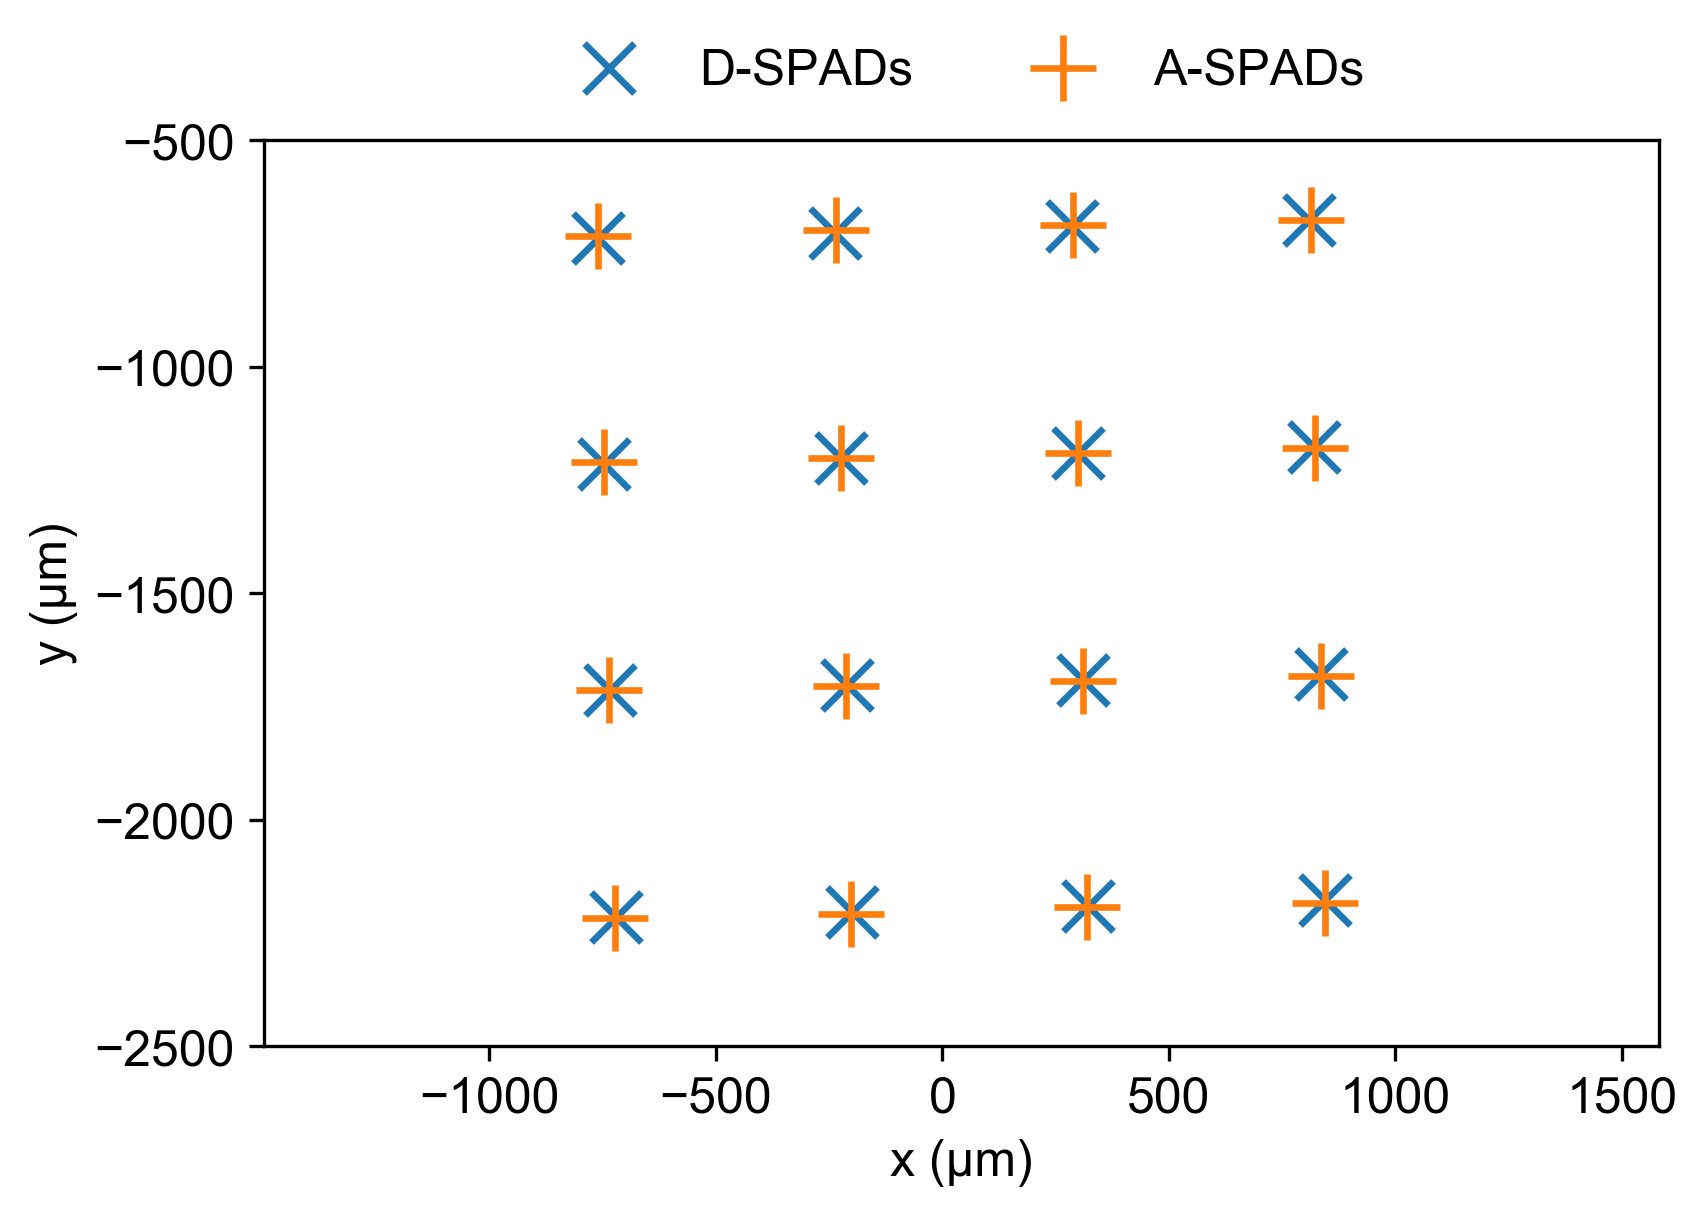
\includegraphics[width=0.9\columnwidth]{figures/2017-05-02_scan_fit_scatter}
\caption{\label{fig:scatter-spad-align}
Experimental SPAD pixel coordinates after fine alignment for the D-SPAD
and A-SPAD arrays obtained with scans of the green LCOS-SLM.
D-SPADs center positions are denoted by 'X'
and A-SPADs center positions are denoted by '+'.
The mean distance between D- and A-SPAD pixels is 2.3~{\micron}.
For details see the notebook
\href{http://nbviewer.jupyter.org/github/tritemio/48-spot-smFRET-PAX-analysis/blob/master/alignment/2017-05-02/48spot alignment-Two\_Mantas-scan\_scatterplot.ipynb}{48spot alignment-Two\_Mantas-scan\_scatterplot}.
}
\end{figure}

\section{ALEX and PAX}
\label{sec:alex_pax}

In ALEX, two alternation time windows, $D_{ex}$ and $A_{ex}$ (respectively the D or A
excitation window) and two detectors (D and A) are involved. This results in four
photon streams noted $D_{ex}D_{em}$, $D_{ex}A_{em}$, $A_{ex}D_{em}$,
$A_{ex}A_{em}$, where the first letter indicates the excitation period and the
second the detection channel. The $A_{ex}D_{em}$ stream only contains
background because there is no fluorescent emission in the D-spectral band
during A-laser excitation and is therefore ignored. For simplicity, we assume in the following that all
quantities have been corrected for
background~\cite{ingargiola_fretbursts:_2016}.

A PAX setup has two detectors (D and A) but only one alternating laser (A).
As in ALEX, two alternation time windows can be defined:
$D_{ex}$, corresponding to the interval during which only the D-laser is on and
${DA}_{ex}$, when both lasers are on. As before this results into four photon
streams noted $D_{ex}D_{em}$, $D_{ex}A_{em}$, $DA_{ex}D_{em}$, $DA_{ex}A_{em}$.
Formally, the only difference with ALEX is that $A_{ex}$ in
ALEX is replaced with $DA_{ex}$. In PAX, however, all
four photon streams contain fluorescent signal. In particular,
$DA_{ex}D_{em}$ contains D-fluorescence due to D-laser excitation (the
corresponding term in ALEX, $A_{ex}D_{em}$, contains only background).
With this
notation,  we can define the total fluorescence signal
during D-excitation (valid in both ALEX and PAX) as:

\begin{equation}
    \Lambda = {F_{D_{ex}D_{em}} + F_{FRET}}
    \label{eq:burstsize_raw}
\end{equation}

\noindent where the $F$ quantities are background-corrected photon counts.
$F_{FRET}$ is the detected acceptor fluorescence due to FRET, computed by
subtracting from $F_{D_{ex}A_{em}}$ the D-leakage in the acceptor channels
($Lk$) and the A-direct-excitation by A-laser
($Dir$)~\cite{lee_accurate_2005}:

\begin{equation}
    F_{FRET} = F_{D_{ex}A_{em}} - Lk - Dir
    \label{eq:F_FRET}
\end{equation}

We also need the usual correction factors
$\gamma$ and $\beta$~\cite{lee_accurate_2005}:

\begin{align}
    \gamma &= \frac{\phi_A \, \eta_{A_{det}}^{A_{em}}}
                   {\phi_D \, \eta_{D_{det}}^{D_{em}}} \label{eq:gamma} \\
    \beta &= \frac{I_{A_{ex}}\sigma_{A_{ex}}^A}{I_{D_{ex}}\sigma_{D_{ex}}^D}
    \label{eq:beta}
\end{align}

\noindent where $\phi_A$, $\phi_D$ are the acceptor and donor quantum yields
and $\eta_{A_{det}}^{A_{em}}$, $\eta_{D_{det}}^{D_{em}}$ are the detection
efficiencies of the D and A signals in the D and A channels.
In eq.~\ref{eq:beta}, $I_{A_{ex}}$ and $I_{D_{ex}}$ are A and D-excitation
intensities, while $\sigma_{A_{ex}}^A$ and $\sigma_{D_{ex}}^D$
are the dye absorption cross-sections at their respective laser wavelengths.
$\beta$ accounts for the difference in D and A-dye excitation rates when
each dye is excited by its respective laser.

We can define the $\gamma$-corrected total signal upon D-excitation
as~\cite{lee_accurate_2005,ingargiola_applying_2017}:

\begin{equation}
    \Lambda_\gamma = {\gamma\,F_{D_{ex}D_{em}} + F_{FRET}}
    \label{eq:burstsize}
\end{equation}
With these definitions, the proximity ratio
$E_{PR}$ and FRET efficiency $E$ are given by the following expression,
valid for both ALEX and PAX:

\begin{align}
    E_{PR} &= \frac{F_{FRET}}{\Lambda} \label{eq:Epr} \\
    E &= \frac{F_{FRET}}{\Lambda_\gamma} \label{eq:E}
\end{align}

By contrast, the expression for the stoichiometry ratio $S$ is slightly
different for ALEX and PAX.
In ALEX, $S$ and its corrected version $S_{\gamma\beta}$ are defined as:

\begin{align}
    S &= \frac{\Lambda}{\Lambda + F_{AexAem}} \label{eq:S} \\
    S_{\gamma\beta} &= \frac{\Lambda_\gamma}
                            {\Lambda_\gamma + {\beta}^{-1}F_{AexAem}}
                            \label{eq:Sgb}
\end{align}

The value $S_{\gamma\beta}$ is always centered around 0.5 for doubly-labeled
species, regardless of FRET efficiency or D and A-excitation intensities.

In PAX, there is no such signal as $F_{A_{ex}A_{em}}$. However, when
the alternation period is sufficiently short to assume that the excitation
intensity doesn't change from one interval to the next
(which is usually the case), an equivalent quantity can be
computed by subtracting the contribution of D-excitation to
$F_{DA_{ex}A_{em}}$:

\begin{equation}
    \tilde{F}_{A_{ex}A_{em}} = F_{DA_{ex}A_{em}} - \frac{w_A}{w_D}F_{D_{ex}A_{em}}
    \label{eq:pax_Faa}
\end{equation}

\noindent where $w_A$ and $w_D$ are the durations of the $DA_{ex}$ and
$D_{ex}$ excitation periods respectively.
Typically the alternation periods have the same duration
(i.e. duty cycle $= 0.5$) and $w_A/w_D = 1$.
Expressions for $S$ and $S_{\gamma\beta}$ defined for ALEX (eq.~\ref{eq:S}
and \ref{eq:Sgb}) can then be used for PAX, with the replacement of
$F_{A_{ex}A_{em}}$ by $\tilde{F}_{A_{ex}A_{em}}$:

\begin{align}
S &= \frac{\Lambda}
          {\Lambda + \tilde{F}_{AexAem}} \label{eq:Spax} \\
S_{\gamma\beta} &= \frac{\Lambda_\gamma}
                        {\Lambda_\gamma + {\beta}^{-1}{\tilde{F}_{AexAem}}}
         \label{eq:Sgb_pax}
\end{align}

Since in PAX experiments the D-excitation is always on, we can use
the signal in $F_{DA_{ex}D_{em}}$ to improve photon statistics.
To derive a modified set of PAX expressions for $E$ and $S$
we start by defining a ``modified'' total FRET signal as:

\begin{align}
    \Lambda_{PAX} &= F_{D_{ex}D_{em}} + F_{DA_{ex}D_{em}}
                     + \alpha^{-1}\,F_{FRET}
    \label{eq:burstsizerawpaxe} \\
    \Lambda_{\gamma,PAX} &= \gamma\,(F_{D_{ex}D_{em}} + F_{DA_{ex}De_{m}})
                            + \alpha^{-1}\,F_{FRET}
    \label{eq:burstsize_paxe}
\end{align}

\noindent where $\alpha = \left( 1 + \frac{w_A}{w_D} \right)^{-1}$ is the
$D_{ex}$ duty cycle (typically, $w_A = w_D$ and $\alpha = 0.5$).
The factor $\alpha^{-1}$ amplifies the $F_{FRET}$ signal in order
to compensate for the additional donor signal $F_{DA_{ex}D_{em}}$.

Based on eq.~\ref{eq:burstsizerawpaxe} and \ref{eq:burstsize_paxe}, we
can write modified PAX expressions for $E$ and $S$:

\begin{align}
    E_{PR,PAX} &= \frac{\alpha^{-1} \, F_{FRET}}{\Lambda_{PAX}} \label{eq:Epr_paxe} \\
    E_{PAX} &= \frac{\alpha^{-1} \, F_{FRET}}{\Lambda_{\gamma,PAX}} \label{eq:Epaxe} \\
    S_{PAX} &= \frac{\Lambda_{PAX}}{\Lambda_{PAX} + \tilde{F}_{A_{ex}A_{em}}}
    \label{eq:Spaxe} \\
    S_{\gamma\beta,PAX} &= \frac{\Lambda_{\gamma,PAX}}
        {\Lambda_{\gamma,PAX} + (\alpha\beta)^{-1}\tilde{F}_{A_{ex}A_{em}}}
    \label{eq:Sgb_paxe}
\end{align}

Eq.~\ref{eq:Epr_paxe}, \ref{eq:Epaxe}, \ref{eq:Spaxe}
and~\ref{eq:Sgb_paxe} contain more photons than the classical expressions
and, therefore, can result in lower shot-noise. However, this effect is
mitigated by the fact that $F_{FRET}$ is multiplied by $\alpha^{-1}$ to
compensate for the additional D signal $F_{DA_{ex}D_{em}}$, and
therefore its shot-noise is amplified.



\subsection{Modified stoichiometry}
\label{sec:Su}

By replacing $\tilde{F}_{A_{ex}A_{em}}$ with $F_{DA_{ex}A_{em}}$ in
eq.~\ref{eq:Spax}, a modified or ``uncorrected stoichiometry'' $S_u$ can
be defined:

\begin{equation}
S_u = \frac{\Lambda}
           {\Lambda + F_{DA_{ex}A_{em}} }
\label{eq:Su}
\end{equation}

This expression avoids subtracting $F_{D_{ex}A_{em}}$ counts from
$F_{DA_{ex}A_{em}}$ (an operation which sums the statistical noise
of these two quantities), therefore improving the overall dispersion
of the ratiometric quantity $S_u$.
As a result, the
$S_u$ distributions are narrower, permitting easier
separation of FRET and D-only population. Note, however, that $S_u$ has a
built-in dependency on the population FRET value, in particular
$S_u$ decreases with increasing $E$.
In this work, even at low FRET values, better separation between
FRET and D-only population was achieved using $S_u$ instead of
$S$. In general, the advantage of $S_u$ over $S$ may change in
other situations, especially when  signal-to-noise and
signal-to-background ratios are large.
Once populations are separated in the $E-S_u$ histogram, one
can use the classical $S$ expression (eq. \ref{eq:Spax}) to compute
gamma factor as described in ref.~\onlinecite{lee_accurate_2005}.
In this work, no attempt was made to recover exact FRET values and
D-A distances, therefore no gamma factor calibration was performed.
However, we address the issue of differences in collection and detection
efficiencies across spots, which can affect such a calibration, in
Section~\ref{sec:perchcorr}.


\section{Individual spot corrections}
\label{sec:perchcorr}

\subsection{Gamma correction}

The gamma-factor of each spot, $\gamma_{sp}$, can be expressed as
the product of an average factor $\gamma_m$ and a spot-specific adjustment
factor $\chi_{sp}$:

\begin{equation}
\gamma_{sp} = \gamma_m \cdot \chi_{sp}
\label{eq:gamma_split}
\end{equation}

$\chi_{sp}$ can be easily computed from measurable
quantities according to the following expression:

\begin{equation}
\chi_{sp} = \frac{{\langle E_{PR,sp} \rangle_N}^{-1} - 1}{{E_{PR,sp}}^{-1} - 1}
\label{eq:chich}
\end{equation}

In eq.~\ref{eq:chich}, $E_{PR,sp}$ is the sub-population
proximity ratio measured in a specific spot, and $ \langle E_{PR,sp} \rangle_N $
is its average over all $N$ spots (here, $N= 48$).

Eq.~\ref{eq:chich} follows from the following relation between $E$
and $E_{PR}$\cite{lee_accurate_2005, ingargiola_applying_2017}:

\begin{equation}
E = f(E_{PR}, \gamma) = \frac{1}{1 + \gamma \left( {E_{PR}}^{-1} - 1 \right)}
\label{eq:EfuncEpr}
\end{equation}

Solving eq.~\ref{eq:EfuncEpr} for $\gamma$, we obtain:

\begin{equation}
\gamma = \frac{{E}^{-1} - 1}{{E_{PR}}^{-1} - 1}
\label{eq:gamma_funcEEpr}
\end{equation}

Formally, we can write $\gamma = \gamma_1 \gamma_2 $, where $\gamma_1$
is associated with a partially corrected
proximity ratio $E_1$ as follows:

\begin{equation}
E_1 = f(E_{PR}, \gamma_1) = \frac{1}{1 + \gamma_1 \left( {E_{PR}}^{-1} - 1 \right)}
\label{eq:E1funcEpr}
\end{equation}

Writing $\gamma_1$ as a function of $E_1$ as in~\ref{eq:gamma_funcEEpr} and
substituting the expression into eq.~\ref{eq:EfuncEpr},
we obtain $E$ as a function of $E_{1}$:

\begin{equation}
E = f(E_1, \gamma_2) = \frac{1}{1 + \gamma_2 \left( {E_1}^{-1} - 1 \right)}
\label{eq:EfuncE1}
\end{equation}

Eq.~\ref{eq:EfuncE1} has the same form as \ref{eq:EfuncEpr}
and~\ref{eq:EfuncE1}. Therefore,
$E$ can be obtained by two subsequent (chained) corrections for $\gamma_1$ and
$\gamma_2$ respectively as in eq.~\ref{eq:EfuncEprE1}.

\begin{equation}
E = f(E_{PR}, \gamma) =  f(E_1, \gamma_2) = f(f(E_{PR}, \gamma_1), \gamma_2)
\label{eq:EfuncEprE1}
\end{equation}

In the multispot case, we apply this property to decompose the gamma
correction into a spot-specific correction and an average correction as
in~\ref{eq:gamma_split}.
In particular, eq.~\ref{eq:chich} directly derives from~\ref{eq:gamma_funcEEpr}
with simple substitutions.

\subsection{Beta correction}

Since, formally eq.~\ref{eq:S} and~\ref{eq:Sgb} have the same form as
$E_{PR}$ and $E$, we can write an expression
equivalent to~\ref{eq:EfuncEpr} for $S$ and
$S_{\gamma\beta}$. Dropping the $\gamma$ subscript, we
obtain:

\begin{equation}
S_{\beta} = \frac{1}{1 + {\beta}^{-1} \left( {S}^{-1} - 1 \right)}
\label{eq:SbfuncS}
\end{equation}

Following the same arguments as in the previous Section,
the beta correction can be expressed as the product of a spot-average
$\beta_m$ and an individual spot correction $\beta_{sp}$:

\begin{equation}
\beta = \beta_m \, \beta_{sp}
\label{eq:beta_factor}
\end{equation}

Similarly to eq.~\ref{eq:chich}, we can compute $\beta_{sp}$ as:

\begin{equation}
\frac{1}{\beta_{sp}} = \frac{{\langle S_{sp} \rangle_{N}}^{-1} - 1}{{S_{sp}}^{-1} - 1}
\label{eq:betach}
\end{equation}

\noindent where $S_{sp}$ is the sub-population non-beta-corrected
stoichiometry  ratio for a specific spot, and $ \langle S_{sp} \rangle_{N} $ is the
average over all $N$
channels (here $N= 48$).

\section{Additional data}
\label{sec:moredata}

Fig.~\ref{fig:alexhist48all22d} shows $E_{PR}$-$S_u$ histograms for the
different channels obtained during the measurement of a 22d DNA sample
(low-FRET). Due to the choice of donor and acceptor excitation powers
during this measurement, the FRET population has a $S_u$ value > 0.5, artificially compressing the histograms in the upper part of
the graph. Nonetheless, it is still possible to distinguish FRET from
D-only bursts, despite the low value of $E_{PR}$ for that sample, allowing
an unbiased estimation of $E_{PR}$, as opposed to what would have happened
in the absence of acceptor excitation~\cite{ingargiola_multispot_2017}.

\begin{figure*}
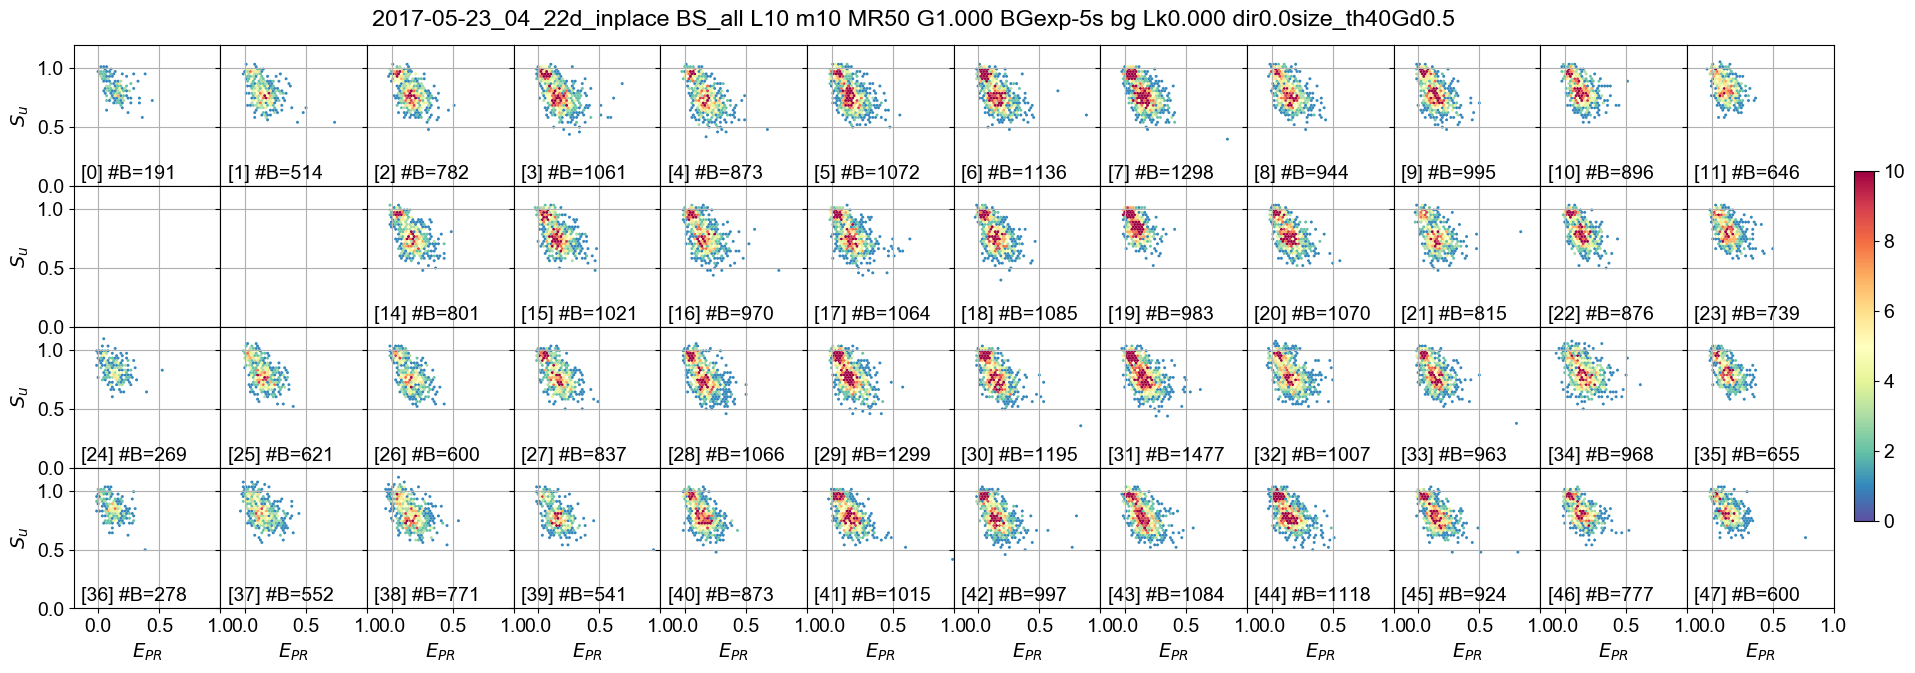
\includegraphics[width=\textwidth]{figures/2017-05-23_04_22d_48spot_alex_hist_Su_all-bursts}
\caption{{\label{fig:alexhist48all22d} $E_{PR}$ versus $S_u$
histograms of all spots for the 22d dsDNA sample. Data analysis and
burst search are identical as in figure~\ref{fig:alexhist48all12d}.
Burst search was performed using all photons with
constant threshold (50~kcps). Burst selection was performed
on the total burst size after background correction, using a threshold of
40 photons. The legend in each subplot
reports spot number in brackets and number of bursts (\#B).
For more details see the notebook
\href{http://nbviewer.jupyter.org/github/tritemio/48-spot-smFRET-PAX-analysis/blob/master/smFRET-PAX\_single\_pop-2017-05-23\_04\_22d.ipynb}{smFRET-PAX\_single\_pop-2017-05-23\_04\_22d}.
}}
\end{figure*}

\nocite{*}
\bibliography{biblio}% Produces the bibliography via BibTeX.

\end{document}
%
% ****** End of file aipsamp.tex ******
